\documentclass[8pt]{beamer}

%%pacotes referentes ao Beamer
%\useoutertheme{split}
%\setbeamertemplate{navigation symbols}{}

%\usetheme{beamertheme}
%\usebeamercolor{beamer-color name}

%\usetheme{Boadilla}
%\usecolortheme{dove}

\usetheme{CambridgeUS}
\usecolortheme{beaver}

% \usetheme{pittsburgh}
% \usecolortheme{dolphin}
%\usecolortheme{dove}
%\usecolortheme{seahorse}

%\usetheme{Montpellier}

%number in figures an tables -- beamer
\setbeamertemplate{caption}[numbered]

%Colocar no description
%[leftmargin=!,labelwidth=\widthof{Turma A}]
	
%pacotes usuais do latex
\usepackage[portuguese]{babel}
\usepackage[utf8]{inputenc}
\usepackage{bm}
\usepackage{graphicx}
\usepackage{subfigure}
\usepackage[round]{natbib}
\usepackage{tikz}
\usetikzlibrary{shapes,arrows}
\usepackage{natbib}
\usepackage{times}
\usepackage{calc} %computes the length of a string
\usepackage{dsfont} %pacote para o 1 estilisado para indicadora
\usepackage{enumerate} %permite fazer uns enumerates diferentes
\usepackage[font=small,labelfont=bf]{caption} %permite colocar um segundo caption
\usepackage{booktabs} % comando \toprule, \midrule e \bottomrule
\usepackage{times} %times new roman font
\usepackage{multirow} %comando \multirow
\usepackage{setspace}
\usepackage{xcolor} %texto colorido
\usepackage{booktabs} %costumized tabs
\usepackage{tikz}
\usepackage{units} %nice fractions

\usetikzlibrary{decorations.pathreplacing}

%código para alinhar a esquerda os itens no description
\defbeamertemplate{description item}{align left}{\insertdescriptionitem\hfill}
\defbeamertemplate{enumerate item}{align left}{\insertdescriptionitem\hfill}



%AMS packages
\usepackage{amsmath}
\usepackage{amsfonts}
\usepackage{amssymb}

%Não quebre linhas
\binoppenalty=\maxdimen
\relpenalty=\maxdimen

%Comandos criados por mim
\DeclareMathOperator*{\argmin}{arg\,min}

\DeclareMathOperator*{\argmax}{arg\,max}


\DeclareMathOperator{\espe}{E}

\DeclareMathOperator{\spann}{span}

\DeclareMathOperator{\cov}{Cov}

\DeclareMathOperator{\vari}{Var}

%Informações para o primeiro slide
\date{}
\title[Medidas Resumo]{Medidas Resumo: \\ Medidas de Posição, Medidas de Dispersão e Quantis}
\author[Gilberto Sassi]{Gilberto Pereira Sassi}
\institute[IME -- UFBA]{Universidade Federal da Bahia \\ Instituto de Matem\'{a}tica e Estat\'{i}stica\\ Departamento de Estat\'{i}stica }

\begin{document}
	
\tikzstyle{decision} = [diamond, draw, fill=blue!20, 
text width=4.5em, text badly centered, node distance=3cm, inner sep=0pt]
\tikzstyle{block} = [rectangle, draw, fill=blue!20, 
text width=5em, text centered, rounded corners, minimum height=4em]
\tikzstyle{line} = [draw, -latex]
\tikzstyle{cloud} = [draw, ellipse,fill=red!20, node distance=3cm,
minimum height=2em]
	
%Slide inicial
\begin{frame}{}
	\maketitle
\end{frame}

\section{Medidas de Posição}

\subsection{Média}

\begin{frame}{Medidas de posição}
  \begin{block}{Medidas Resumo}
   Obter um ou mais números que sintetizem toda informação na amostra. 
   
   Consideraremos duas classes de medidas resumo: medidas de posição e medidas de dispersão.
  \end{block}

  \begin{block}{Medidas de Posição}
   Moda, Média e Mediana.
  \end{block}
  
  \begin{block}{Média}
    Suponha que os valores de uma variável $X$ em uma amostra sejam $x_1, \dots, x_n$, então a média é calculada por
    \begin{align*}
     \bar{x} = \dfrac{x_1+ \dots + x_n}{n}.
   \end{align*}
  \end{block}
\end{frame}

\begin{frame}{Exemplo}
   Considere as notas finais ($X$) da Turma 1 de Estatística Aplicada à Saúde: 6,91; 7,85; 7,68; 8,64; 7,21; 8,04; 8,68; 4,37; 6,41; 7,89. Calcule a nota final média dessa turma.
   \vfill
   
   \textbf{Solução:} Então a nota final média da Turma 1 é 
   \begin{align*}
    \bar{x} &= \dfrac{6,91 +7,85+ 7,68+ 8,64+ 7,21+ 8,04+ 8,68+ 4,37+ 6,41+ 7,89}{10}\\
    &= 7,37.
   \end{align*}

\end{frame}



\begin{frame}{Uso da Tabela de Distribuiçao de Frequência: Caso Discreto}
 Se $X$ é uma variável quantitativa discreta com a seguinte tabela de distribuição de frequência
 
 {\tiny
  \begin{table}
   \centering
   \begin{tabular}{l|cccc}
    \toprule[0.05cm]
    $X$ & Frequência & Frequência Relativa (Proporção) & Porcentagem\\
    \midrule[0.05cm]
    $x_1$ & $n_1$ & $f_1=\nicefrac{n_1}{n}$ & $100\cdot f_1\%$\\ \hline
    $\vdots$ & $\vdots$ & $\vdots$ & $\vdots$ \\ \hline
    $x_k$ & $n_k$ & $f_k=\nicefrac{n_k}{n}$ & $100\cdot f_k\%$\\ \midrule[0.05cm]
    Total & $n=n_1+\cdots+n_k$ & $1,00$ & $100\%$\\ \bottomrule[0.05cm]
   \end{tabular}
  \end{table}
 }
 
 então a média de $X$ é dada por
 \begin{align*}
  \bar{x} &= \dfrac{ \overbrace{x_1+\cdots+x_1}^{n_1\mbox{ vezes}} + \overbrace{x_2+\cdots+x_2}^{n_2\mbox{ vezes}} + \cdots + \overbrace{x_k+\cdots+x_k}^{n_k\mbox{ vezes}} }{n}\\
  &= {\color{red} \dfrac{n_1 \cdot x_1 + n_2 \cdot x_2 + \cdots + n_k \cdot x_k}{n}} \\
  &= \overbrace{\dfrac{n_1}{n}}^{f_1} \cdot x_1 + \overbrace{\dfrac{n_2}{n}}^{f_2} \cdot x_2 + \cdots + \overbrace{\dfrac{n_k}{n}}^{f_k} \cdot x_k \\
  &= {\color{blue} f_1 \cdot x_1 + f_2 \cdot x_2 + \cdots + f_k \cdot x_k}
 \end{align*}

 
\end{frame}


\begin{frame}{Exemplo}
 Retome a variável Número de Filhos ($Z$) da amostra com 36 funcionário da companhia MB cuja distribuição de frequência é dada por
 
 {\tiny
 \begin{table}
  \centering
  \begin{tabular}{l|ccc}
    \toprule[0.05cm]
    Número de Filhos & Frequência & Frequência Relativa (Propoção) & Porcentagem\\
    \midrule[0.05cm]
    0 & 20 & 0,5556 & 55,56\% \\
    1 & 5 & 0,1389 & 13,89\% \\
    2 & 7 & 0,1944 & 19,44\% \\
    3 & 3 & 0,0833 & 8,33\% \\
    4 & 0 & 0,00 & 0,00\% \\
    5 & 1 & 0,0278 & 2,78\% \\ \midrule[0,05cm]
    Total & 36 & 1,00 & 100\% \\ \bottomrule[0,05cm]
  \end{tabular}
 \end{table}
 }
 
Calcule a média da variável $Z$.

{\small
\textbf{Solução:} Então a média é dada por
\begin{align*}
 \bar{z} &=  \dfrac{20 \cdot 0 + 1 \cdot 5 + 2\cdot 7 + 3 \cdot 3 + 1 \cdot 5}{36}\\
 &= 0,92,
\end{align*}
ou de forma alternativa
\begin{align*}
 \bar{z} &= 0,5556 \cdot 0 + 0,1389 \cdot 1 + 0,1944 \cdot 2 + 0,0833 \cdot 3 + 0,0278 \cdot 5\\
 &= 0,92.
\end{align*}
}

\end{frame}


\begin{frame}{Uso da Tabela de Distribuiçao de Frequência: Caso Contínuo}
 \begin{block}{Observação}
  Para variáveis quantiativas contínuas também podemos usar a Tabela de Distribuição de Frequência. 
  
  Note que nesse caso teremos uma {\color{red} aproximação} da média, pois perdemos informação ao agregar os valores 
  em classes.
 \end{block}
 
 Considere a variável quantitativa contínua $X$ cuja tabela de distribuição de frequência é
 
 {\tiny
 \begin{table}
  \centering
  \begin{tabular}{l|ccc}
    \toprule[0.05cm]
    X & Frequência & Proporção & Porcentagem \\ \midrule[0.05cm]
    $l_1 |--- l_2$ & $n_1$ & $f_1=\nicefrac{n_1}{n}$ & $100\cdot f_1 \%$ \\ \hline
    $l_2 |--- l_3$ & $n_2$ & $f_1=\nicefrac{n_2}{n}$ & $100\cdot f_2 \%$ \\ \hline
    $\vdots$ & $\vdots$ & $\vdots$ & $\vdots$\\ \hline
    $l_k |--- l_{k+1}$ & $n_k$ & $f_1=\nicefrac{n_k}{n}$ & $100\cdot f_k \%$ \\ \midrule[0.05cm]
    Total & $n=n_1+\cdots+n_k$ & $1,00$ & $100\%$\\ \bottomrule[0.05cm]
  \end{tabular}
 \end{table}
 }

 Usamos a simplificação: todos os valores observados de $X$ que pertencem a classe $l_i |--- l_{i+1}, i =1, \dots, k$ são bem aproximados por $\dfrac{l_i+l_{i+1}}{2}$.
\end{frame}

\begin{frame}{Exemplo}
 Considere a variável quantativa contínua salário ($S$) da seção de orçamentos da companhia MB cuja tabela de distribuição de frequência é 
 
 {\tiny
  \begin{table}
   \centering
   \begin{tabular}{l|ccc|c}
    \toprule[0.05cm]
   \multicolumn{1}{c|}{$S$} & Frequência & Frequência Relativa & Porcentagem & Ponto Médio \\ \midrule[0.05cm]
    $4 |--- 8$ & $10$ & $\nicefrac{10}{36}=0,2778$ & $27,78 \%$ & $\nicefrac{(4+8)}{2} = 6$ \\
    $8 |--- 12$ & $12$ & $\nicefrac{12}{36}=0,3333$ & $33,33 \%$ & $\nicefrac{(8+12)}{2} = 10$\\
    $12 |--- 16$ & $8$ & $\nicefrac{8}{36}=0,2222$ & $22,22 \%$ &  $\nicefrac{(12+16)}{2} = 14$\\
    $16 |--- 20$ & $5$ & $\nicefrac{5}{36}=0,1389$ & $13,89 \%$ & $\nicefrac{(16+20)}{2} = 18$\\
    $20 |--- 24$ & $1$ & $\nicefrac{1}{36}=0,0278$ & $2,78 \%$ & $\nicefrac{(20+24)}{2} = 22$\\ \midrule[0.05cm]
   \multicolumn{1}{c|}{Total} & 36 & 1,00 & 100\% & $--$ \\ \bottomrule[0.05cm]
   \end{tabular}
  \end{table}
 }
 
 \textbf{Solução:} Então a média salarial pode ser {\color{red} aproximada} por
 \begin{align*}
  \bar{s} &= \dfrac{10\cdot 6 + 12 \cdot 10 + 8 \cdot 14 + 5 \cdot 18 + 1 \cdot 22}{36}\\
  &= 0,2778 \cdot 6 + 0,3333 \cdot 10 + 0,2222 \cdot 14 + 0,1389 \cdot 18 + 0,0278 \cdot 22\\
  &= 11,22.
 \end{align*}

 {\color{blue} Note que a média salarial sem usar a tabela de distribuição de frequência é $11,12$}
\end{frame}

\subsection{Moda}

\begin{frame}{}
 Geralmente usamos essa medida de posição com variáveis quantitativas discretas.
 \begin{block}{Moda}
  Realização mais frequente de uma variável.
 \end{block}

 \begin{block}{Exemplo}
 Considere a variável Número de Filhos ($Z$) da seção de orçamentos da companhia MB cuja tabela de distribuição é dada por

  {\tiny
 \begin{table}
  \centering
  \begin{tabular}{l|ccc}
    \toprule[0.05cm]
    Número de Filhos & Frequência & Frequência Relativa (Propoção) & Porcentagem\\
    \midrule[0.05cm]
    0 & 20 & 0,5556 & 55,56\% \\
    1 & 5 & 0,1389 & 13,89\% \\
    2 & 7 & 0,1944 & 19,44\% \\
    3 & 3 & 0,0833 & 8,33\% \\
    4 & 0 & 0,00 & 0,00\% \\
    5 & 1 & 0,0278 & 2,78\% \\ \midrule[0,05cm]
    Total & 36 & 1,00 & 100\% \\ \bottomrule[0,05cm]
  \end{tabular}
 \end{table}
 }
 
 Qual a moda?
 
 \textbf{Solução:} A moda da variável Número de Filhos é 0.
 \end{block}
\end{frame}

\subsection{Mediana}

\begin{frame}{}
  \begin{block}{Mediana}
   Realização que ocupa a posição central da série de observações, ou seja, $50\%$ das observações estão abaixo da mediana.
  \end{block}

  \begin{block}{Algoritmo para cáculo}
  Seja $X$ uma variável quantitativa com valores observados $x_1, \dots, x_n$.
  \begin{enumerate}[1)]
   \item Ordenar os valores  do menor ao maior:
   \begin{align*}
    x_{(1)} \quad \leq \quad x_{(2)} \quad \leq \quad \cdots \quad \leq \quad x_{(n)}.
   \end{align*}
   \item \begin{align*}
          md(x) = \begin{cases}
                   x_{\left( \frac{n+1}{2}\right)}, & \mbox{se } n \mbox{ é ímpar},\\
                  \dfrac{ x_{\left( \frac{n}{2}\right)}+x_{\left( \frac{n}{2}+1\right)} }{2}, & \mbox{se } n \mbox{ é par},\\
                  \end{cases}
         \end{align*}

  \end{enumerate}
  \end{block}
  Note que $x_{(1)}$ representa o menor valor de $X$ na amostra, $x_{(2)}$ representa o segundo menor valor de $X$ na amostra, $x_{(3)}$ representa o terceiro menor valor de $X$ na amostra, e assim por 
  diante. Chamamos $x_{(1)}, x_{(2)}, \cdots, x_{(n)}$ de estatísticas de ordem.
\end{frame}

\begin{frame}{Exemplo}

{\small
  \begin{block}{Exemplo: tamanho amostral par.}
   Considere a variável quantitativa $X$ com valores observados: $2,8,4$. Calcule a mediana.
   
   \textbf{Solução:} Primeiro ordenamos os valores
   \begin{align*}
    x_{(1)} = 2 \qquad \leq \qquad x_{(2)}=4  \qquad \leq \qquad x_{(3)}=8.
   \end{align*}
  
  O tamanho amostral é $n=3$, então
  \begin{align*}
   md(x) &= x_{\left( \frac{3+1}{2} \right)} = x_{(2)} = 4.
  \end{align*}
  \end{block}
  
    \begin{block}{Exemplo: tamanho amostral ímpar.}
   Considere a variável quantitativa $Y$ com valores observados: $1,2,3,8$. Calcule a mediana.
   
   \textbf{Solução:} Primeiro ordenamos os valores
   \begin{align*}
    x_{(1)} = 1 \qquad \leq \qquad x_{(2)}=2  \qquad \leq \qquad x_{(3)}=3 \qquad \leq \qquad x_{(4)}=8.
   \end{align*}
  
  O tamanho amostral é $n=4$, então
  \begin{align*}
   md(x) &= \dfrac{ x_{\left( \frac{4}{2} \right)} + x_{\left( \frac{4}{2} +1\right)} }{2} = \dfrac{x_{(2)} + x_{(3)} }{2}=\dfrac{2+3}{2} = 2,5.
  \end{align*}
  \end{block}

}

\end{frame}

\begin{frame}{Uso da tabela de distribuiçao de frequência: caso discreto}

 {\scriptsize
Considere a variável Número de Filhos com tabela de distribuição de frequência dada por


 \begin{table}
  \centering
  \begin{tabular}{l|ccc}
    \toprule[0.05cm]
    Número de Filhos & Frequência & Frequência Relativa (Propoção) & Porcentagem\\
    \midrule[0.05cm]
    0 & 20 & 0,5556 & 55,56\% \\
    1 & 5 & 0,1389 & 13,89\% \\
    2 & 7 & 0,1944 & 19,44\% \\
    3 & 3 & 0,0833 & 8,33\% \\
    4 & 0 & 0,00 & 0,00\% \\
    5 & 1 & 0,0278 & 2,78\% \\ \midrule[0,05cm]
    Total & 36 & 1,00 & 100\% \\ \bottomrule[0,05cm]
  \end{tabular}
 \end{table}

 
 Calcule a mediana.
 
 
 \textbf{Solução:} Primeiro encontramos as estatísticas de ordem
 \begin{align*}
  &x_{(1)}=x_{(2)}=\cdots=x_{(20)} = 0\\
  &x_{(21)} = x_{(22)} = x_{(23)} = x_{(24)} = x_{(25)}=1\\
  &x_{(26)} = x_{(27)} =  x_{(28)} = x_{(29)} = x_{(30)} = x_{(31)} = x_{(32)} = 2\\
  &x_{(33)} = x_{(34)} = x_{(35)} = 3\\
  &x_{(36)} = 5
 \end{align*}
 O tamanho amostral $n=36$ é par, então $md(x) = \dfrac{ x_{\left( \frac{36}{2} \right)}+x_{\left( \frac{36}{2} +1\right)}}{2} = \dfrac{ x_{(18)}+x_{(19)}}{2} = \dfrac{0+0}{2}=0$.
}
\end{frame}

\begin{frame}{Uso da tabela de distribuiçao de frequência: caso contínuo}


\begin{block}{Observação}
  Para variáveis quantiativas contínuas também podemos usar a Tabela de Distribuição de Frequência. 
  
  Note que nesse caso teremos uma {\color{red} aproximação} da mediana, pois perdemos informação ao agregar os valores 
  em classes.
 \end{block}

 \begin{block}{Exemplo}
 
 Considere a variável salário ($S$) da seção de orçamentos da companhia MB cuja tabela de distribuição de frequência é 
   \begin{table}
   \centering
   \begin{tabular}{l|ccc|c}
    \toprule[0.05cm]
    \multicolumn{1}{c|}{$S$} & Frequência & Frequência Relativa & Porcentagem & Ponto Médio \\ \midrule[0.05cm]
    $4 |--- 8$ & $10$ & $\nicefrac{10}{36}=0,2778$ & $27,78 \%$ & $\nicefrac{(4+8)}{2} = 6$ \\
    $8 |--- 12$ & $12$ & $\nicefrac{12}{36}=0,3333$ & $33,33 \%$ & $\nicefrac{(8+12)}{2} = 10$\\
    $12 |--- 16$ & $8$ & $\nicefrac{8}{36}=0,2222$ & $22,22 \%$ &  $\nicefrac{(12+16)}{2} = 14$\\
    $16 |--- 20$ & $5$ & $\nicefrac{5}{36}=0,1389$ & $13,89 \%$ & $\nicefrac{(16+20)}{2} = 18$\\
    $20 |--- 24$ & $1$ & $\nicefrac{1}{36}=0,0278$ & $2,78 \%$ & $\nicefrac{(20+24)}{2} =22$\\ \midrule[0.05cm]
    \multicolumn{1}{c|}{Total} & 36 & 1,00 & 100\% & $--$ \\ \bottomrule[0.05cm]
   \end{tabular}
  \end{table}
  Calcule a mediana. 
  \end{block}
\end{frame}

\begin{frame}{Solução exemplo}
  
  \textbf{Solução:} Primeiro encontramos as estatísticas de ordem
  \begin{align*}
   &s_{(1)} = s_{(2)}=s_{(3)}=x_{(4)}=s_{(5)}=s_{(6)}=s_{(7)}=s_{(8)}=s_{(9)}=s_{(10)}=6\\
   &s_{(11)} = s_{(12)}=s_{(13)}=s_{(14)}=s_{(15)}=s_{(16)}=s_{(17)}=s_{(18)}=s_{(19)}=s_{(20)}=s_{(21)}=s_{(22)}=10\\
   &s_{(23)} = s_{(24)}=s_{(25)}=s_{(26)}=s_{(27)}=s_{(28)}=s_{(29)}=s_{(30)}=14\\
   &s_{(31)} = s_{(32)}=s_{(33)}=s_{(34)}=s_{(35)}=18\\
   &s_{(36)} = 22
  \end{align*}
 
 Note que o tamanho amostral $n=36$ é par, logo
 \begin{align*}
  md(s)&=\dfrac{ s_{\left(\frac{36}{2}\right)}+s_{\left(\frac{36}{2}+1\right)}}{2}\\
  &=\dfrac{ s_{(18)}+s_{(19)}}{2}\\
  &= \dfrac{10+10}{2}\\
  &=10.
 \end{align*}
 
 {\color{blue} Note que 10 é uma aproximação para a mediana de salário cujo valor é 10,165 (usando os 36 valores observados na amostra). }
\end{frame}

\subsection{Exemplo: Medidas de Posição}

\begin{frame}{Exemplo}
 Um editor deseja estudar o número de erros de impressão de um livro. Para isso ele escolheu uma amostra de 50 páginas de um livro com a seguinte tabela de distribuição de frequência
 
 {\tiny
 \begin{table}
  \centering
  \begin{tabular}{l|ccc}
  \toprule[0.05cm]
    Erro de impressão ($X$) & Frequência & Frequência Relativa & Porcentagem \\ \midrule[0.05cm]
    0 & 25 & $\nicefrac{25}{50}=0,5$ & $0,5\cdot 100=50\%$\\
    1 & 20 & $\nicefrac{20}{50}=0,4$ & $0,4\cdot 100=40\%$\\
    2 & 3 & $\nicefrac{3}{50}=0,06$ & $0,06\cdot 100=6\%$\\
    3 & 1 & $\nicefrac{1}{50}=0,02$ & $0,02\cdot 100=2\%$\\
    4 & 1 & $\nicefrac{1}{50}=0,02$ & $0,02\cdot 100=2\%$\\ \midrule[0.05cm]
    Total & 50 & 1,00 & 100\% \\ \bottomrule[0.05cm]
  \end{tabular}
 \end{table}
 }
 
 \begin{enumerate}[a)]
  \item Qual o número médio de erros por página?
  \item E o número mediano?
  \item Faça uma representação gráfica para a variável $X$.
  \item Se o livro tem 500 páginas, qual o número aproximado de erros de impressão?
 \end{enumerate}
\end{frame}

\begin{frame}{Solução -- exemplo.}
 \begin{enumerate}[a)]
  \item 
  \begin{align*}
   \bar{x} &=\dfrac{ 25 \cdot 0 + 20 \cdot 1 + 3 \cdot 2 + 1 \cdot 3 + 1 \cdot 4}{50}\\
   &= 0,5 \cdot 0 + 0,4 \cdot 1 + 0,06 \cdot 2 + 0,02 \cdot 3 + 0,02 \cdot 4\\
   &=0,66
  \end{align*}

  \item Primeiro encontramos as estaísticas de ordem
  \begin{align*}
   &x_{(1)} = x_{(2)} = x_{(3)} = \cdots = x_{(25)} = 0; \qquad x_{(26)} = x_{(27)} = x_{(28)} =  \cdots = x_{(45)} = 1\\
   &x_{(46)} = x_{(47)} = x_{(48)}  = 2; \qquad x_{(49)} = 3; \qquad x_{(50)} = 4
  \end{align*}

  Note que $n=50$ é par, logo 
  \begin{align*}
   md(x) =\dfrac{ x_{\left( \frac{50}{2} \right)}+x_{\left( \frac{50}{2} +1\right)}}{2} =\dfrac{ x_{(25)}+x_{(26)}}{2} = \dfrac{0+1}{2} = 0,5.
  \end{align*}
  
  \item[d)] Se um página tem aproximadamente $0,66$ erros, então 500 páginas tem aproximadamente $500 \cdot 0,66 = 330$ erros de impressão.
 \end{enumerate}

\end{frame}

\begin{frame}{Solução -- exemplo: continuação}
\begin{enumerate}[a)]
 \item[c)] \textbf{Interpretação:} Notamos que a maioria das páginas tem até dois erros de impressão.
 
 \begin{figure}
  \centering
  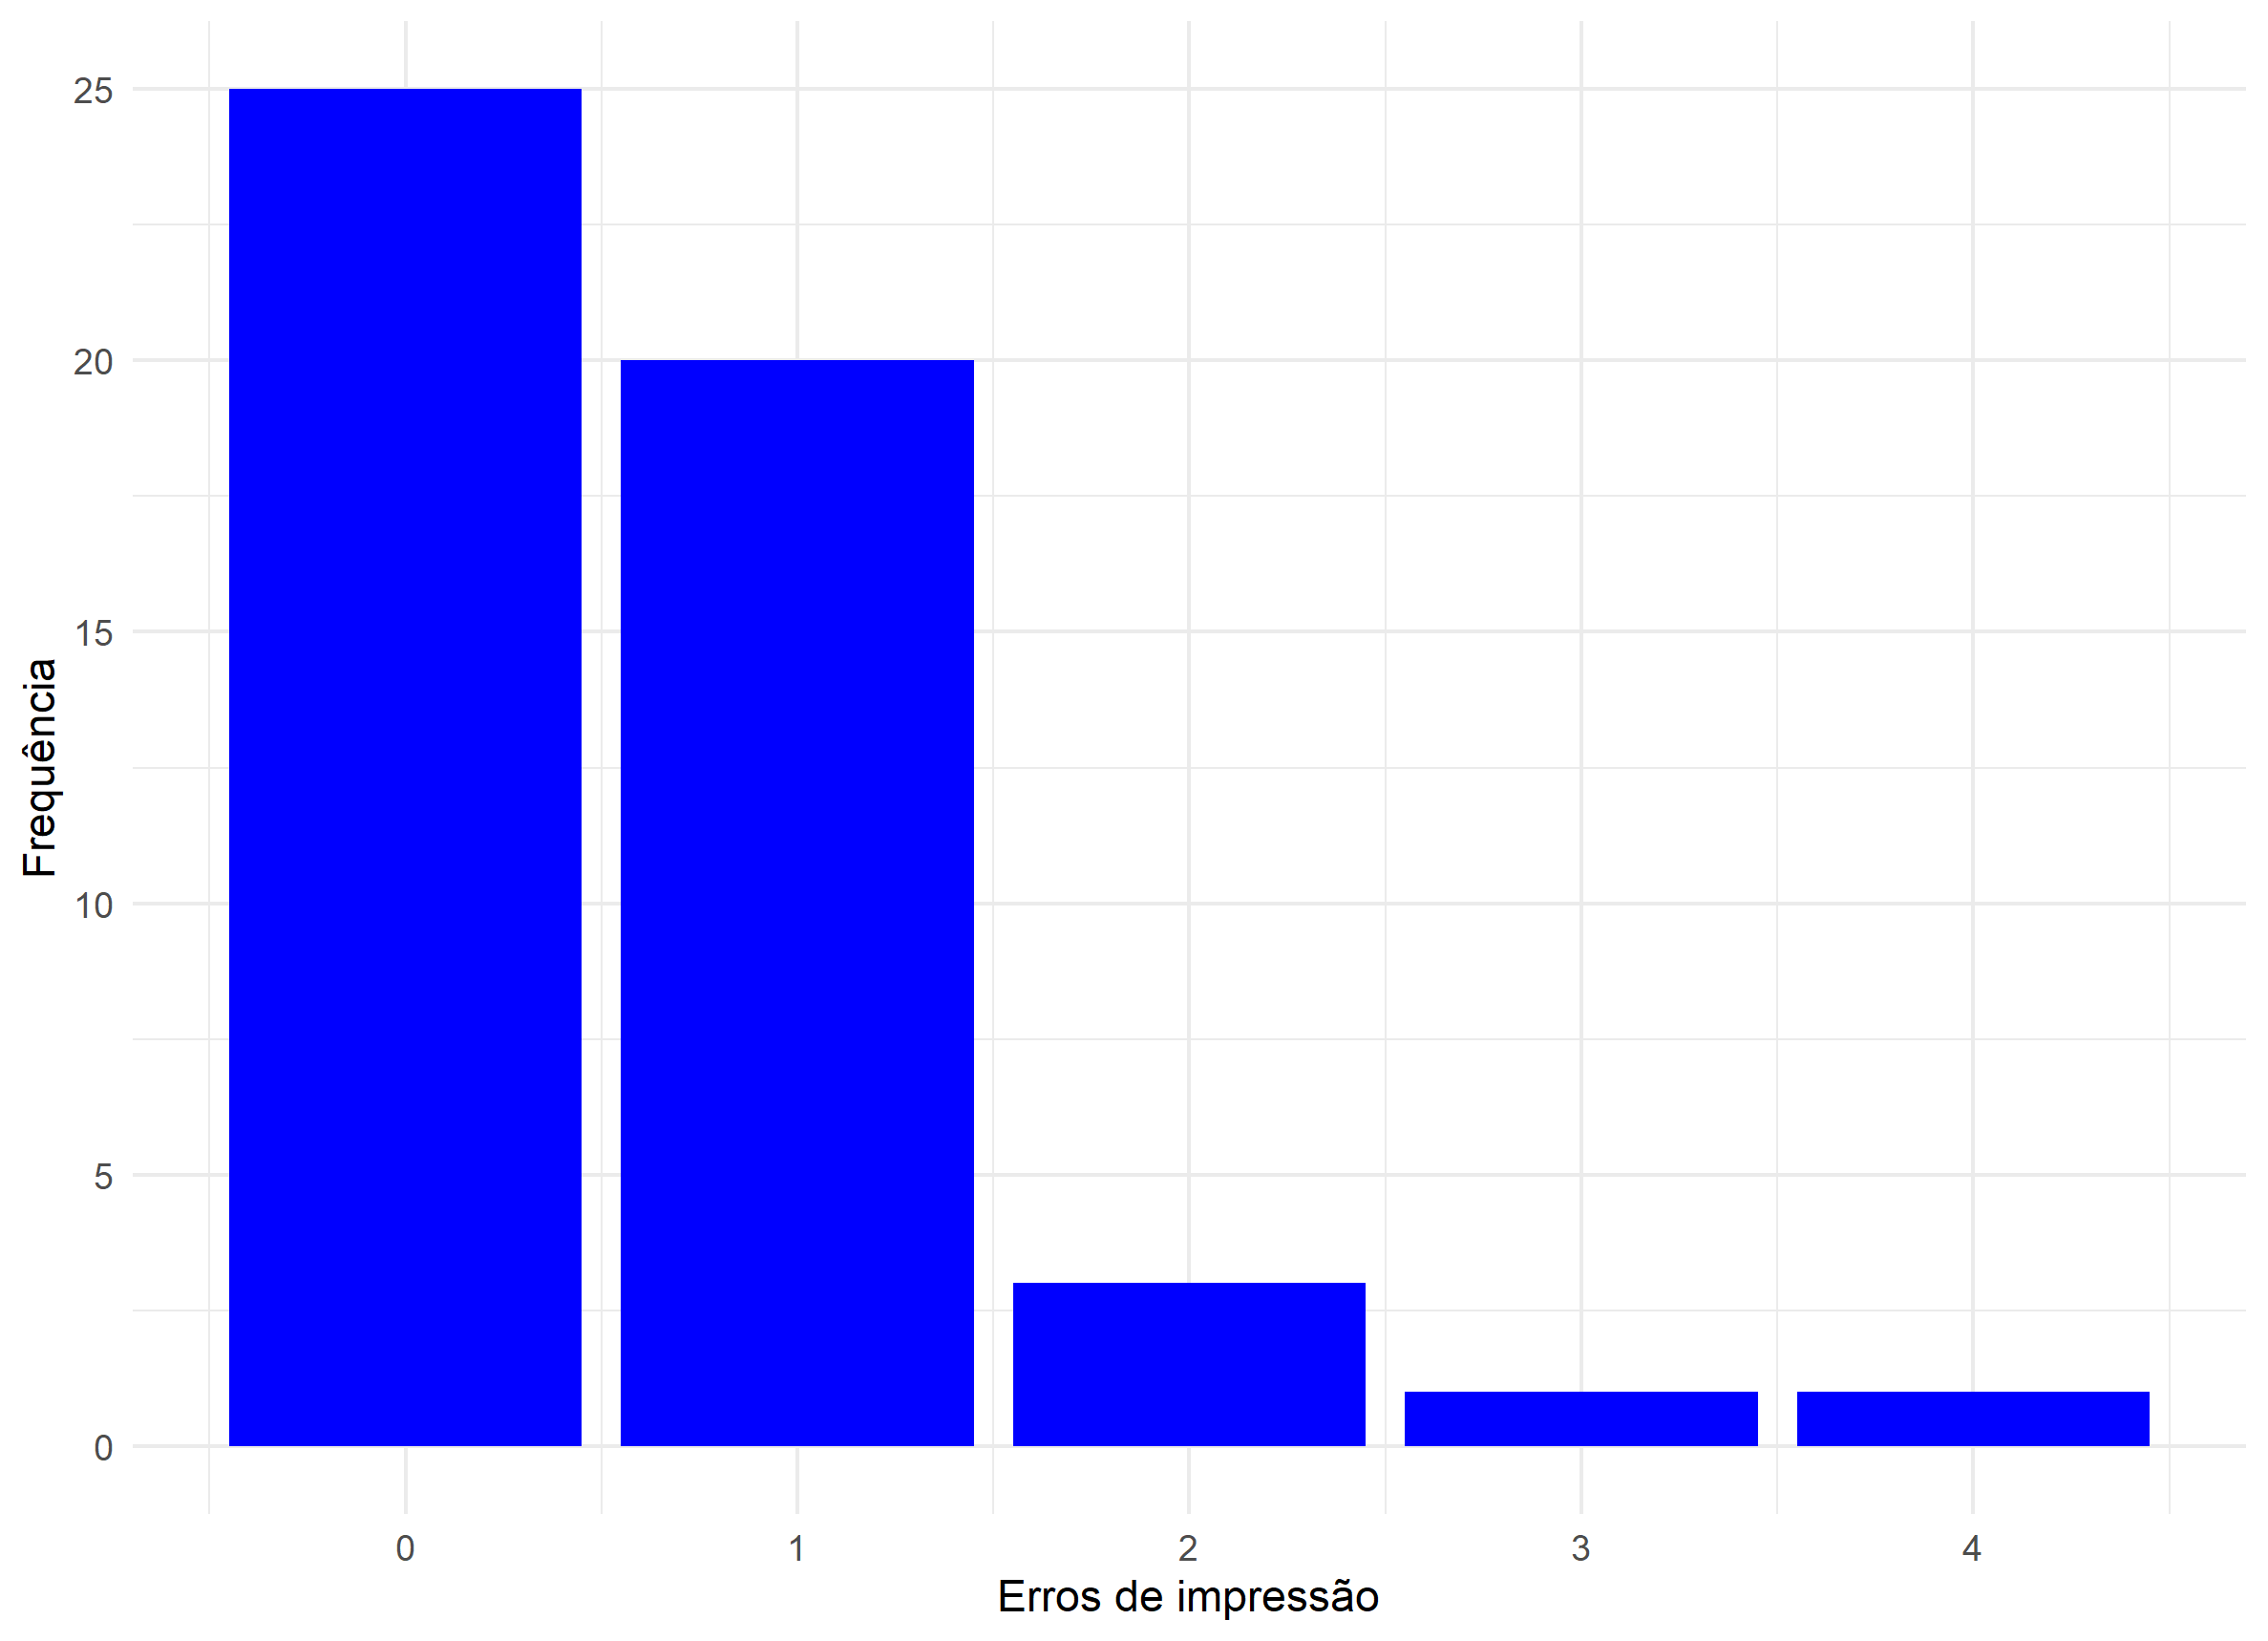
\includegraphics[width=10cm]{erros_livro.png}
 \end{figure}

\end{enumerate}
\end{frame}

\section{Medidas de dispersão}

\begin{frame}{Motivação}
 \begin{block}{Observação}
  Note que a medida de posição pode mascarar a informação de como os dados estão dispersos.
 \end{block}
 
 \begin{block}{Exemplo de motivação.}
  Um grupo de cinco alunos fizeram uma bateria de 5 testes, obtendo os seguintes resultados:
  \begin{table}
   \centering
   \begin{tabular}{c|ccccc|c}
   \toprule[0.05cm]
    Teste & \multicolumn{5}{|c|}{Notas} & Representação da variável \\ \midrule[0.05cm]
    A & 3 & 4 & 5 & 6 & 7 & $X$ \\
    B & 1 & 3 & 5 & 7 & 9 & $Y$ \\
    C & 5 & 5 & 5 & 5 & 5 & $Z$ \\
    D & 4 & 5 & 5 & 6 & 5 & $W$\\ \bottomrule[0.05cm]
   \end{tabular}
  \end{table}
  {\color{magenta} Exercício para casa:} verifique que a moda, média e mediana de $X$, $Y$, $Z$ e $W$ são iguais 5.
 \end{block}
\end{frame}

\begin{frame}{Motivação -- continuação}
 \begin{figure}
  \centering
  \begin{tikzpicture}[scale=0.8]
   \draw[->] (-1,0) -- (11,0);
   \node[right] at (11,0) {$X$};
   \foreach \i in {1,2,3,4,5,6,7,8,9} \filldraw[black] (\i,0) circle (0.025cm);
   \foreach \i in {1,2,3,4,5,6,7,8,9} \node[below] at (\i,0) {\i};
   \foreach \i in {3,4,5,6,7} \filldraw[blue] (\i,0.2) circle (0.035cm);
   \draw[->] (-1,1) -- (11,1);
   \node[right] at (11,1) {$Y$};
   \foreach \i in {1,2,3,4,5,6,7,8,9} \filldraw[black] (\i,1) circle (0.025cm);
   \foreach \i in {1,2,3,4,5,6,7,8,9} \node[below] at (\i,1) {\i};
   \foreach \i in {1,3,5,7,9} \filldraw[blue] (\i,1+0.2) circle (0.035cm);
   \draw[->] (-1,2) -- (11,2);
   \node[right] at (11,2) {$Z$};
   \foreach \i in {1,2,3,4,5,6,7,8,9} \filldraw[black] (\i,2) circle (0.025cm);
   \foreach \i in {1,2,3,4,5,6,7,8,9} \node[below] at (\i,2) {\i};
   \foreach \i in {1,2,3,4,5} \filldraw[blue] (5,2+\i*0.2) circle (0.035cm);
   \draw[->] (-1,4) -- (11,4);
   \node[right] at (11,4) {$W$};
   \foreach \i in {1,2,3,4,5,6,7,8,9} \filldraw[black] (\i,4) circle (0.025cm);
   \foreach \i in {1,2,3,4,5,6,7,8,9} \node[below] at (\i,4) {\i};
   \filldraw[blue] (4,4+0.2) circle (0.035cm);
   \filldraw[blue] (6,4+0.2) circle (0.035cm);
   \foreach \i in {1,2,3} \filldraw[blue] (5,4+\i*0.2) circle (0.035cm);
   \draw[red, line width=0.5cm, opacity=0.15] (5,-1) -- (5,5);
   \node[above] at (5,5) {$\underbrace{\mbox{Média, Moda e Mediana}}_{\downarrow}$};
  \end{tikzpicture}
  \caption{Representação gráfica para as variáveis $X$, $Y$, $Z$, $W$.}
  \label{fig:dispersao}
 \end{figure}

\end{frame}

\begin{frame}{Desvio Médio}
\begin{block}{Limitação das medidas de posição}
 As variáveis $X$, $Y$, $Z$ e $W$ tem a mesma média, mediana e moda, mas na Figura~\ref{fig:dispersao} percebemos que as quatro variáveis não são semelhantes. Algumas variáveis tem valor mais acumulado
 em torno da média (mediana ou moda) enquanto outras variáveis tem valores mais ``heterogêneos''.
\end{block}

 \begin{block}{Idea para superar a limitação das medidas de posição}
 Considere uma variável quantitativa com valores observados $x_1, \dots, x_n$ e média $\bar{x}$, então
 \begin{enumerate}[i.]
  \item Calcule a distância (em valor absoluto) entre os valores observados e uma medida de posição (geralmente a média): $\left\vert x_1 - \bar{x} \right\vert$, $\left\vert x_2 - \bar{x} \right\vert$, $\cdots$, $\left\vert x_n - \bar{x} \right\vert$;
  \item Considere um valor representativo dessas distâncias, isto é, uma medida de posição de $\{\left\vert x_1-\bar{x} \right\vert,$ $ \left\vert x_2-\bar{x} \right\vert, \dots, \left\vert x_n-\bar{x} \right\vert$ $\}$.
 \end{enumerate}
 {\color{magenta} Se o valor obtido em ii. for pequeno os valores estão concentrados em torno da medida de posição (média) e são homogêneos. }
 
 Finalmente, podemos o Desvio Médio:
 \begin{align*}
  dm(x) = \dfrac{\left\vert x_1-\bar{x} \right\vert + \left\vert x_2-\bar{x} \right\vert+\cdots+\left\vert x_n-\bar{x} \right\vert}{n}.
 \end{align*}
 Note que usamos a média como medida de posição em ii.
 \end{block} 
\end{frame}

\begin{frame}{Variância e Desvio Padrão}

{\tiny
 \begin{block}{Idea para superar a limitação das medidas de posição}
 Considere uma variável quantitativa com valores observados $x_1, \dots, x_n$ e média $\bar{x}$, então
 \begin{enumerate}[i.]
  \item Calcule a distância (ao quadrado) entre os valores observador e uma medida de posição (geralmente a média): $\left( x_1 - \bar{x} \right)^2$, $\left( x_2 - \bar{x} \right)^2t$, $\cdots$, $\left( x_n - \bar{x} \right)^2t$;
  \item Considere um valor representativo dessas distâncias ao quadrado, isto é, uma medida de posição de $\{\left( x_1-\bar{x} \right)^2,$ $ \left( x_2-\bar{x} \right)^2, \dots, \left( x_n-\bar{x} \right)^2\}$ 
 \end{enumerate}
 {\color{magenta} Se o valor obtido em ii. for pequeno os valores estão concentrados em torno da medida de posição (média) e são homogêneos. } 
 
 Finalmente, podemos introduzir a Variância:
 \begin{align*}
  Var(x) = \dfrac{\left( x_1-\bar{x} \right)^2 + \left( x_2-\bar{x} \right)^2+\cdots+\left( x_n-\bar{x} \right)^2}{n}.
 \end{align*}
 Note que usamos a média como medida de posição em ii.
 
 Para manter a mesma unidade de $X$, é comum usar o Desvio Padrão
 \begin{align*}
  DP(x)  =\sqrt{ \vari(x)}.
 \end{align*}
 \end{block}  
 
 \begin{block}{Motivação}
  Em nosso exemplo de motivação temos que
  \begin{table}
   \centering
   \begin{tabular}{llll}
    $\vari(x) = 2$ & $\vari(y)=8$ & $\vari(z)=0$ & $\vari(w)=0,4 $\\
    $DP(x) = 1,4$ & $DP(y)=2,8$ & $DP(z)=0$ & $DP(w)=0,6 $\\
    $dm(x) = 1,2$ & $dm(y)=2,4$ & $dm(z)=0$ & $dm(w)=0,4$
   \end{tabular}
  \end{table}
  e notamos que as variáveis não são semelhantes (valores são dispersos de forma diferente).
 \end{block}

}
\end{frame}

\begin{frame}{Exemplo}

{\small
   Considere as notas finais ($X$) da Turma 1 de Estatística Básica A: 6,91; 7,85; 7,68; 8,64; 7,21 Calcule a nota final média dessa turma.
   \vfill
   
   \textbf{Solução:} Primeiramente, calculamos a média
   \begin{align*}
    \bar{x} = \dfrac{6,91+ 7,85+ 7,68 +8,64 +7,21}{5} = 7,66
   \end{align*}
   
   
   Então, o desvio médio é 
   \begin{align*}
    dm(x) &= \dfrac{\left\vert6,91 -\bar{x}\right\vert+\left\vert7,85-\bar{x}\right\vert+ \left\vert7,68-\bar{x}\right\vert+ 
    \left\vert8,64-\bar{x}\right\vert+ \left\vert7,21-\bar{x}\right\vert}{5}\\
    &= \dfrac{\left\vert6,91 -7,66\right\vert+\left\vert7,85-7,66\right\vert+ \left\vert7,68-7,66\right\vert+ 
    \left\vert8,64-7,66\right\vert+ \left\vert7,21-7,66\right\vert}{5} \\
    &= 0,48
   \end{align*}
  e a variância é 
  \begin{align*}
   \vari(x) &= \dfrac{(6,91 -\bar{x})^2+(7,85-\bar{x})^2+ (7,68-\bar{x})^2+ 
    (8,64-\bar{x})^2+ (7,21-\bar{x})^2}{5} \\
    &= \dfrac{(6,91 -7,66)^2+(7,85-7,66)^2+ (7,68-7,66)^2+ 
    (8,64-7,66)^2+ (7,21-7,66)^2}{5}\\
    &= 0,35
  \end{align*}
 e o desvio padrão é dado por $DP=\sqrt{0,35} = 0,59$.

}
\end{frame}

\begin{frame}{Uso da tabela de distribuiçao de frequência: caso discreto}

{\tiny
Considere a variável Número de Filhos com tabela de distribuição de frequência dada por


 \begin{table}
  \centering
  \begin{tabular}{l|ccc}
    \toprule[0.05cm]
    Número de Filhos & Frequência & Frequência Relativa (Propoção) & Porcentagem\\
    \midrule[0.05cm]
    0 & 20 & 0,5556 & 55,56\% \\
    1 & 5 & 0,1389 & 13,89\% \\
    2 & 7 & 0,1944 & 19,44\% \\
    3 & 3 & 0,0833 & 8,33\% \\
    4 & 0 & 0,00 & 0,00\% \\
    5 & 1 & 0,0278 & 2,78\% \\ \midrule[0,05cm]
    Total & 36 & 1,00 & 100\% \\ \bottomrule[0,05cm]
  \end{tabular}
 \end{table}

 Já calculamos a média anteriormente: $\bar{x} = 0.92$.
 Então, o desvio médio é dado por
 \begin{align*}
  dm(z) &= \dfrac{20\cdot \left\vert0-0,92\right\vert+5\cdot \left\vert1-0,92\right\vert+7\cdot \left\vert2-0,92\right\vert+3\cdot \left\vert3-0,92\right\vert+0\cdot \left\vert4-0,92\right\vert+1\cdot \left\vert5-0,92\right\vert}{36}\\
  &= 1,02
 \end{align*}
 e a variância é dada por
 \begin{align*}
  \vari(z) &= \dfrac{20\cdot (0-0,92)^2+5\cdot (1-0,92)^2+7\cdot (2-0,92)^2+3\cdot (3-0,92)^2+0\cdot (4-0,92)^2+1\cdot (5-0,92)^2}{36}\\
  &= 1,52
 \end{align*}
  e o desvio padrão é $\sqrt{\vari(z)} = 1,23$.
}
\end{frame}

\begin{frame}{Uso da Tabela de Distribuiçao de Frequência: Caso Contínuo}
\begin{block}{Observação}
  Para variáveis quantiativas contínuas também podemos usar a Tabela de Distribuição de Frequência. 
  
  Note que nesse caso teremos uma {\color{red} aproximação} das medidas de dipersão, pois perdemos informação ao agregar os valores 
  em classes.
 \end{block}

  Considere a variável quantativa contínua salário ($S$) da seção de orçamentos da companhia MB cuja tabela de distribuição de frequência é 
 
 {\tiny
  \begin{table}
   \centering
   \begin{tabular}{l|ccc|c}
    \toprule[0.05cm]
    \multicolumn{1}{c|}{$S$} & Frequência & Frequência Relativa & Porcentagem & Ponto Médio \\ \midrule[0.05cm]
    $4 |--- 8$ & $10$ & $\nicefrac{10}{36}=0,2778$ & $27,78 \%$ & $\nicefrac{(4+8)}{2} = 6$ \\
    $8 |--- 12$ & $12$ & $\nicefrac{12}{36}=0,3333$ & $33,33 \%$ & $\nicefrac{(8+12)}{2} = 10$\\
    $12 |--- 16$ & $8$ & $\nicefrac{8}{36}=0,2222$ & $22,22 \%$ &  $\nicefrac{(12+16)}{2} = 14$\\
    $16 |--- 20$ & $5$ & $\nicefrac{5}{36}=0,1389$ & $13,89 \%$ & $\nicefrac{(16+20)}{2} = 18$\\
    $20 |--- 24$ & $1$ & $\nicefrac{1}{36}=0,0278$ & $2,78 \%$ & $\nicefrac{(20+24)}{2} = 22$\\ \midrule[0.05cm]
    \multicolumn{1}{c|}{Total} & 36 & 1,00 & 100\% & $--$ \\ \bottomrule[0.05cm]
   \end{tabular}
  \end{table}
 }
 
 Calcule o desvio médio, a variância e o desvio padrão. 
\end{frame}

\begin{frame}{Continuação -- exemplo}

{\tiny

Já vimos anteriormente, que a média salarial pode ser aproximada por 11,22. Então,
 \begin{description}
  \item[Desvio Médio]
  \begin{align*}
   dm(s) &= \dfrac{10\cdot \left\vert6-11,22\right\vert+12\cdot \left\vert10-11,22\right\vert+8\cdot \left\vert14-11,22\right\vert+5\cdot \left\vert18-11,22\right\vert+1\cdot \left\vert22-11,22\right\vert}{36}\\
   &=3,72;
  \end{align*}
  
  \item[Variância]
  \begin{align*}
   \vari(s) &= \dfrac{10\cdot (6-11,22)^2+12\cdot (10-11,22)^2+8\cdot (14-11,22)^2+5\cdot (18-11,22)^2+1\cdot (22-11,22)^2}{36}\\
   &= 19,40;
  \end{align*}

  \item[Desvio Padrão]
  \begin{align*}
   DP(s) = \sqrt{\vari(s)} = \sqrt{19,40} = 4,40.
  \end{align*}

 \end{description}

}
\end{frame}

\section{Quantis}

\begin{frame}{Quantis}


 \begin{block}{Ideia}
  Outra abordagem para medidas de posição de forma semelhante a mediana, substituindo $50\%$ por $100\cdot p\%$.
 \end{block}
 
 \begin{block}{Definição}
  Dizemos que um número $q(p)\in \mathbb{R}$ é quantil de ordem $p$ ou $p$-quantil se $100\cdot p\%$ das observações $x_1, \dots, x_n$ forem menores que $q(p)$. 
 \end{block}
 
 \begin{block}{Alguns quantis importantes e seus nomes particulares}
  \begin{description}
   \item[$q(0,25)$] Primeiro Quartil ($q_1$);
   \item[$q(0,5)$] Segundo Quartil ($q_2$) -- sinônimo de mediana;
   \item[$q(0,75)$] Terceiro Quartil ($q_3$).
  \end{description}
 \end{block}

\end{frame}

\begin{frame}{Algoritmo para cálculo de quantis}
 
 Seja $X$ uma variável quantitativa com $x_1, \dots, x_n$ seus valores observados na amostra. 
 \vfill
 
  \begin{enumerate}[i.]
   \item Ordene os valores do menor ao valor (encontre as estatísticas de ordem)
   \begin{align*}
    x_{(1)} \quad \leq \quad x_{(2)} \quad \leq \quad \cdots \quad \leq \quad x_{(n)}
   \end{align*}
   em que $x_{(1)}$ é o menor valor em $\{x_1, \dots, x_n\}$, $x_{(2)}$ é o segundo menor valor em $\{x_1, \dots, x_n\}$, $x_{(3)}$ é o terceiro menor valor em $\{x_1, \dots, x_n\}$, e assim prosseguimos até
   $x_{(n)}$: o último menor valor em $\{x_1, \dots, x_n\}$
   \vfill
   
   \item 
   \begin{align*}
    q(p) = \begin{cases}
            x_{\left((n+1)\cdot p \right)}, & \mbox{se } (n+1)\cdot p \mbox{ é número inteiro},\\
            \dfrac{x_{\left(\lfloor(n+1)\cdot p\rfloor \right)} + x_{\left( \lceil(n+1)\cdot p \rceil \right)}}{2}, & \mbox{se } (n+1)\cdot p \mbox{ não é número inteiro}.
           \end{cases}
   \end{align*}
   em que $\lfloor \cdot \rfloor$ é a função ``arredonda para baixo'' e $\lceil \cdot \rceil$ é a função ``arredonda para cima''.
  \end{enumerate}
\end{frame}


\begin{frame}{Exemplo}
 
  Considere a variável quantitativa $X$ com os seguinte valores observados: 15, 5, 3, 8, 10, 2, 7, 11, 12. Calcule o primeiro, o segundo e terceiro quartis.
  
  \textbf{Solução:} Primeiro encontramos as estatísticas de ordem:
  \begin{align*}
   &x_{(1)}  = 2 \quad \leq \quad x_{(2)}  = 3 \quad \leq \quad x_{(3)}  = 5 \quad \leq \quad x_{(4)}  = 7 \\
   &x_{(5)}  = 8 \quad \leq \quad x_{(6)}  = 10 \quad \leq \quad x_{(7)}  = 11 \quad \leq \quad x_{(8)}  = 12 \quad \leq \quad x_{(9)}  = 15
  \end{align*}
  
  Os quartis são dados por
  \begin{description}
   \item[$q_1$] Note que $(n+1)\cdot 0,25 = (9+1)\cdot 0,25 = 2,5$, e $\lfloor 2,5 \rfloor = 2$ e $\lceil 2,5 \rceil = 3$. Então,
   \begin{align*}
    q_1 = \dfrac{x_{(2)}+x_{(3)}}{2} = \dfrac{3+5}{2} = 4;
   \end{align*}

   \item[$q_2$] Note que $(n+1)\cdot 0,5 = (9+1)\cdot 0,5 = 5$. Então,
   \begin{align*}
    q_2 = x_{(5)} = 8;
   \end{align*}
   
   \item[$q_3$] Note que $(n+1)\cdot 0,75 = (9+1)\cdot 0,75 = 7,5$, e $\lfloor 7,5 \rfloor = 7$ e $\lceil 7,5 \rceil = 8$. Então,
   \begin{align*}
    q_3 = \dfrac{x_{(7)}+x_{(8)}}{2} = \dfrac{11+12}{2} = 11,5.
   \end{align*}
  \end{description}

\end{frame}

\subsection{Intervalo Interquartílico}

\begin{frame}{Intervalo Interquartílico}

\begin{block}{Ideia}
 Se a distância entre $q_1$ e $q_3$ for pequena, então os valores da variável estão concentrados em uma região. 
\end{block}

\begin{figure}
 \centering
  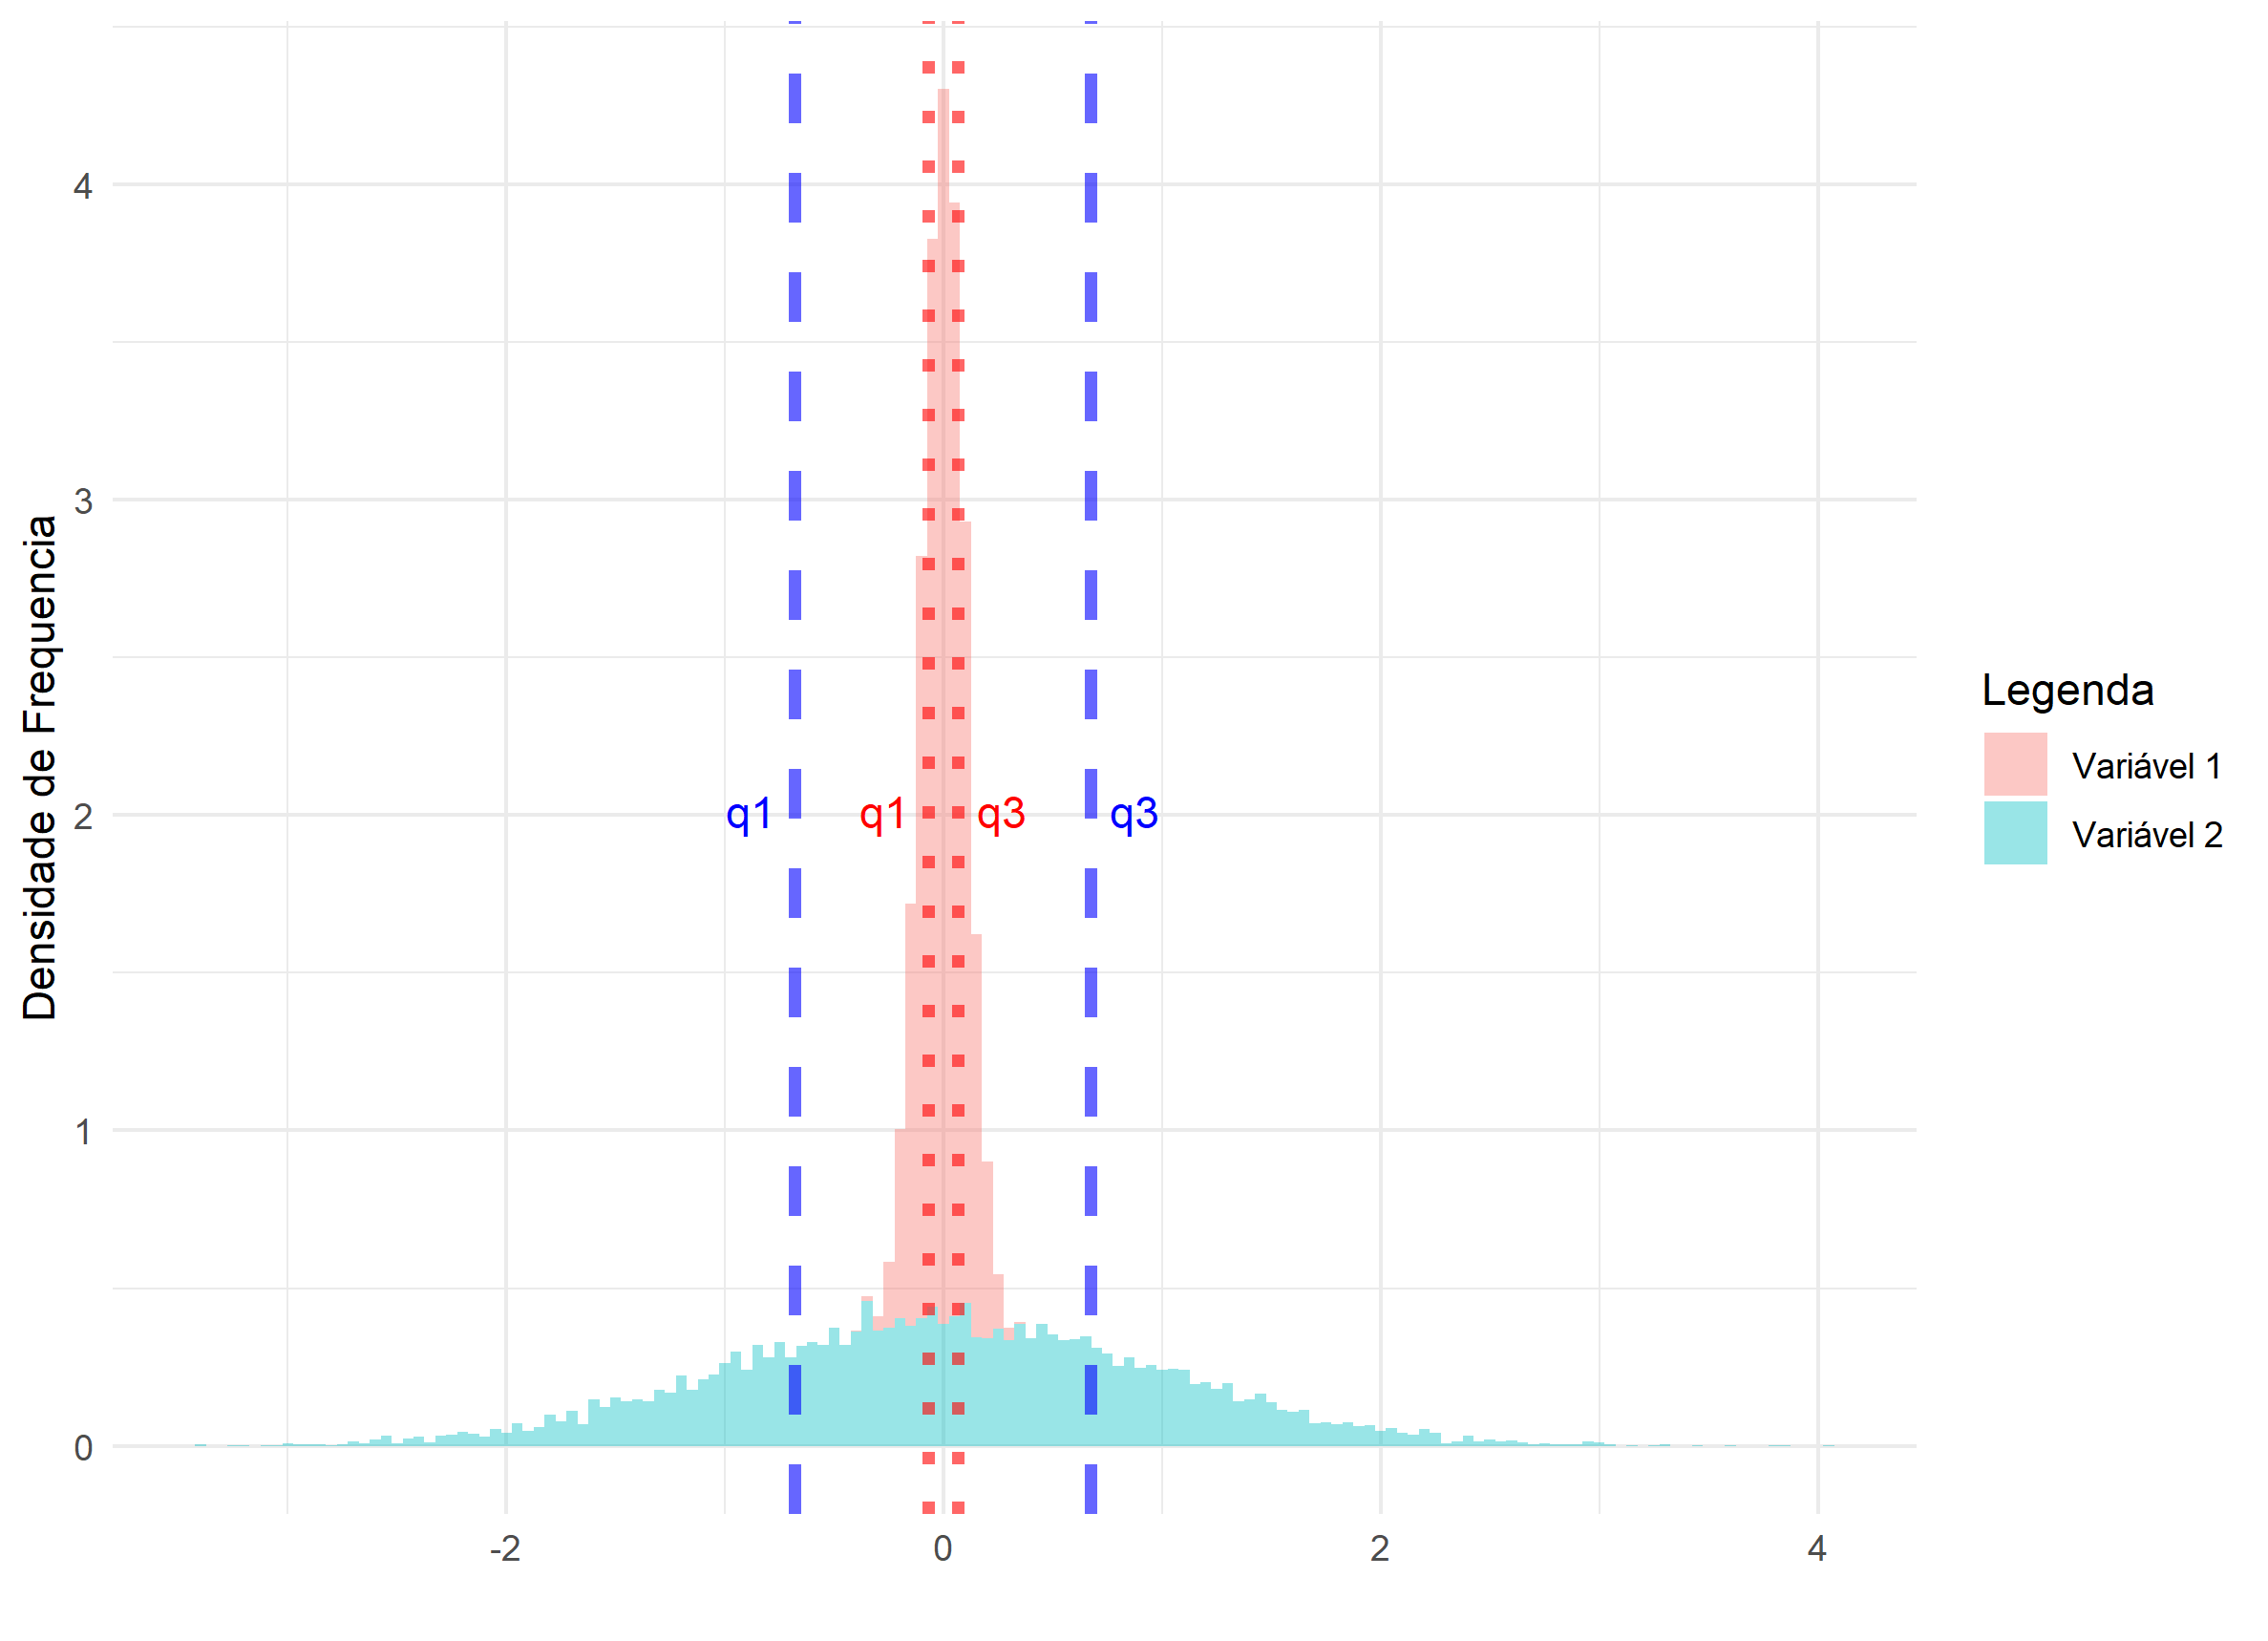
\includegraphics[height=6cm]{motivacao_dq.png}
\end{figure}

\end{frame}

\begin{frame}

\begin{block}{Definição}
 Seja $X$ uma variável quantitativa com valores observados $x_1, \dots, x_n$, então o intervalo interquartílico é dado por
 \begin{align*}
  dq = q_3-q_1
 \end{align*}
\end{block}


\begin{block}{Exemplo}
 Considere a variável quantitativa $X$ com os seguintes valores observados: 15, 5, 3, 8, 10, 2, 7, 11, 12. Calcule o intervalo interquartílico.
 
 \textbf{Solução:} Já calculamos o primeiro e terceiro quartis para essa variável e essa amostra, então
 \begin{align*}
  dq = q_3 - q_1= 11,5 - 4 = 7,5.
 \end{align*}
\end{block}
\end{frame}


\section{Diagrama de Caixa}

\begin{frame}{Diagrama de Caixa ou Boxplot}
 O diagrama de caixa tem o seguinte aspecto
 \begin{figure}
  \begin{tikzpicture}[scale = 0.5]
   \draw[->] (0,-1) -- (0,10);
   \node[left] at (0,1) {LI};
   \node[left] at (0,3) {$q_1$};
   \node[left] at (0,4) {$q_2$};
   \node[left] at (0,5) {$q_3$};
   \node[left] at (0,7) {LS};
   \filldraw[black] (0,1) circle (0.08);
   \filldraw[black] (0,3) circle (0.08);
   \filldraw[black] (0,4) circle (0.08);
   \filldraw[black] (0,5) circle (0.08);
   \filldraw[black] (0,7) circle (0.08);
   \filldraw[black] (2,0) circle (0.08);
   \draw (1.8,1) -- (2.2,1);
   \draw (2,1) -- (2,3);
   \draw (1,3) -- (3,3);
   \draw (1,3) -- (1,5);
   \draw (3,3) -- (3,5);
   \draw (1,5) -- (3,5);
   \draw (1,4) -- (3,4);
   \draw (2,5) -- (2,7);
   \draw (1.8,7) -- (2.2,7);
   \filldraw (2,8) circle (0.08);
   \node[right] at (2,0) {Ponto exterior};
   \node[right] at (2,8) {Ponto exterior};
  \end{tikzpicture}
 \end{figure}

\end{frame}

\begin{frame}{Diagrama de Caixa ou Boxplot}
 Em que
 \begin{description}
  \item[Limite Superior] $LS = q_3 + 1,5 \cdot dq$;
  \vfill
  
  \item[Limite Inferior] $LI = q_1 - 1,5 \cdot dq$;
  \vfill
  
  \item[Ponto Adjacente] Todos os valores da variável entre $LI$ e $LS$;
  \vfill
  
  \item[Ponto Exterior] Todos os valores da variável que não estão entre $LI$ e $LS$. Estes valores da variável são provavelmente destoantes que precisam de atenção do pesquisador;
 \end{description}

\end{frame}

%\begin{frame}{Diagrama de Caixa ou Boxplot}
% Considere a variável quantitativa $X$ com os seguintes valores observados: 15, 5, 3, 8, 10, 2, 7, 11, 12. Desenhe o diagrama de caixa.
% 
% \begin{figure}
%  \centering
%  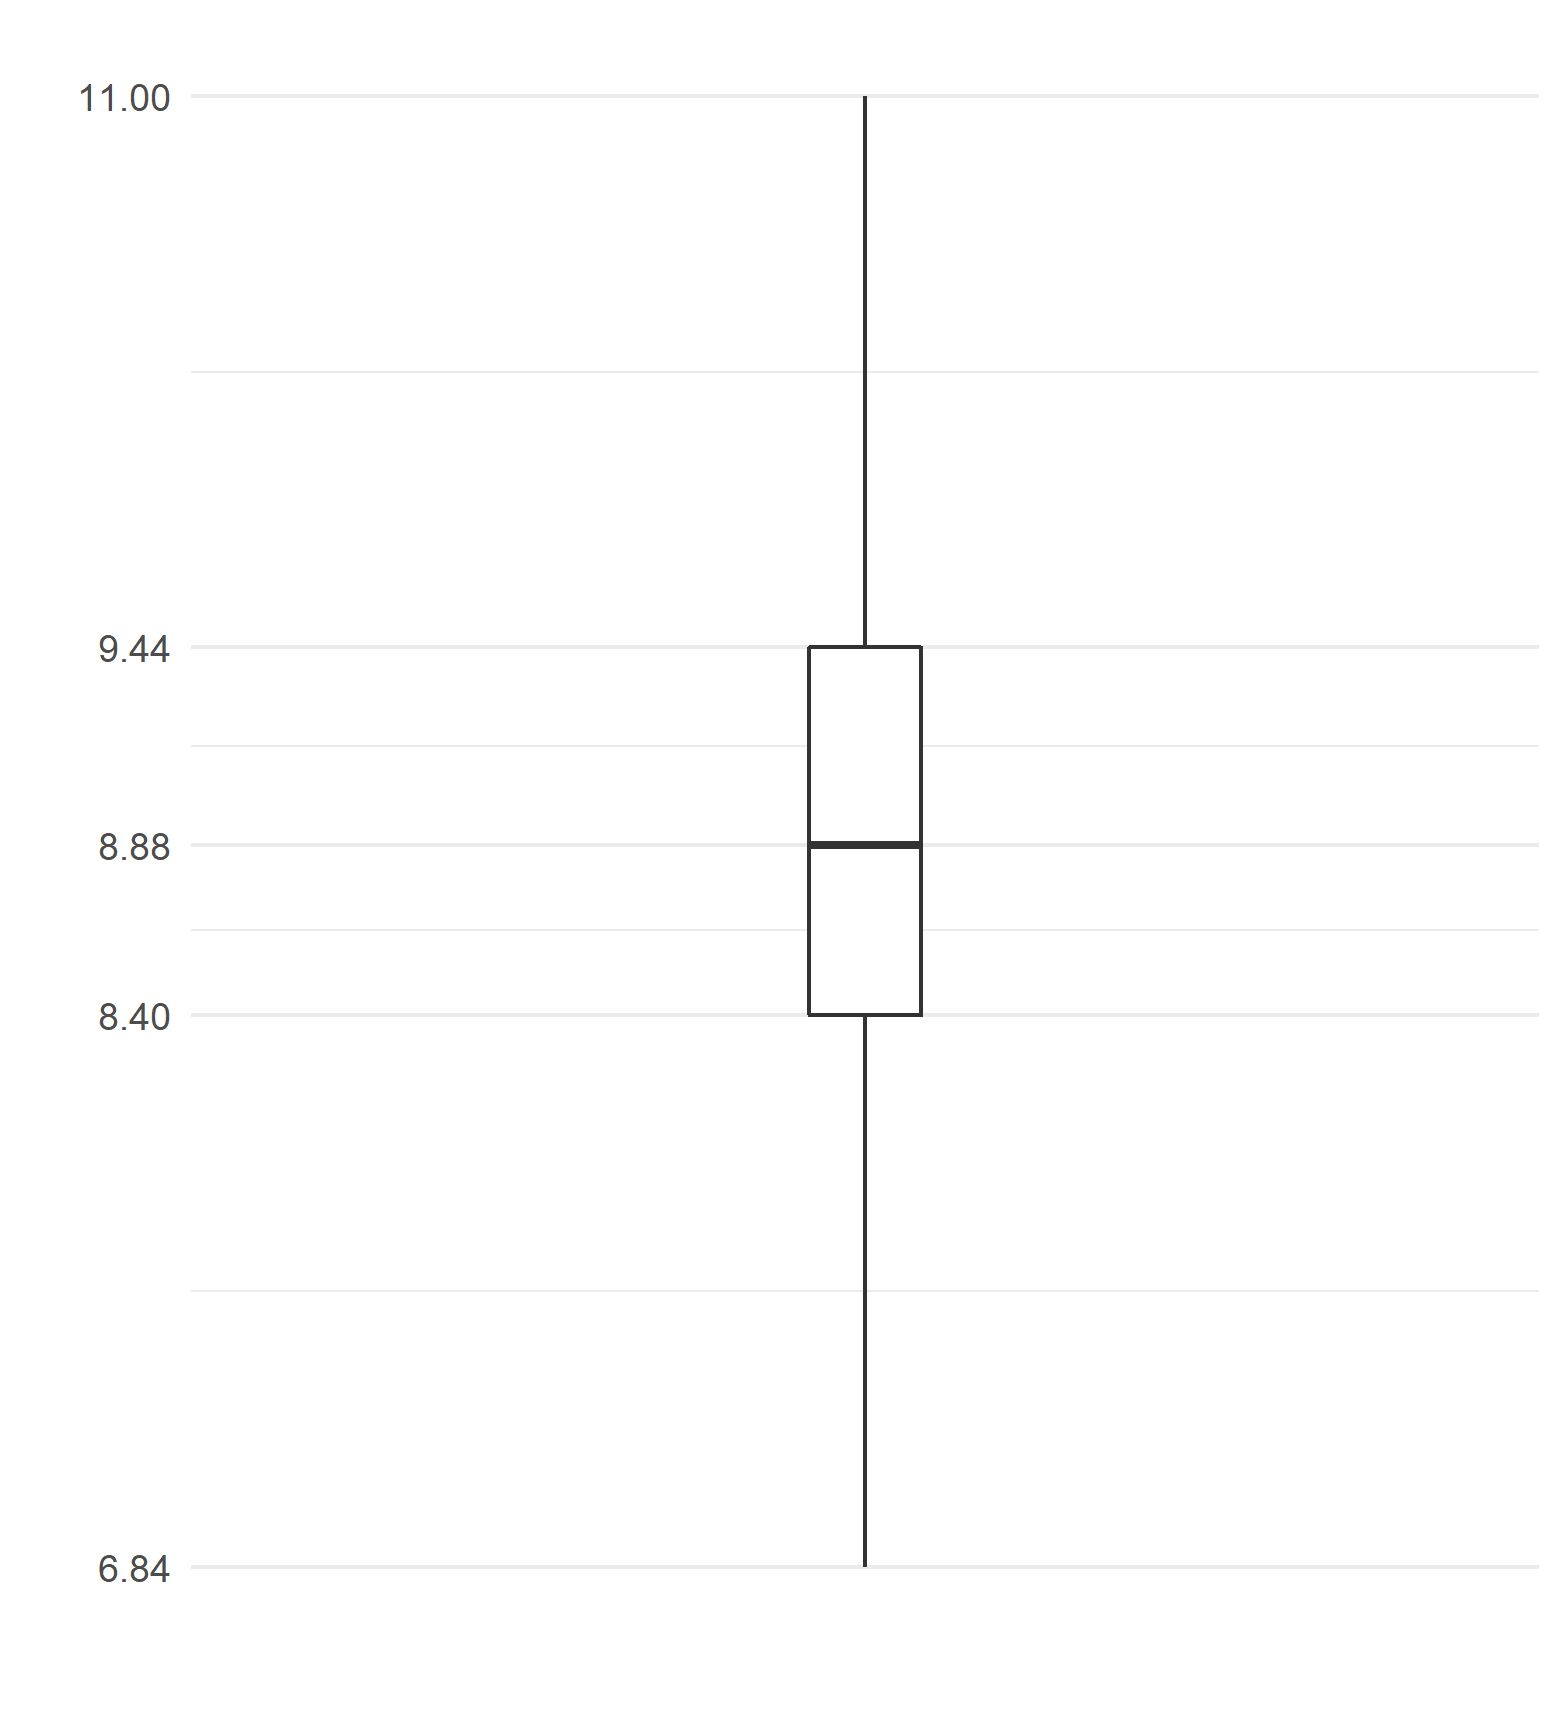
\includegraphics[height = 3cm]{boxplot.png}
% \end{figure}
%
% \begin{description}
%  \item[$q_1$] $4$;
%  \item[$q_2$] $8$;
%  \item[$q_3$] $11,5$;
%  \item[LI] $0,25$;
%  \item[LS] $22,75$;
%  \item[Pontos Exteriores] Não existe.
% \end{description}
%
%\end{frame}

\subsection{Assimetria}

\begin{frame}{Exemplo 1}
	Considere as notas da Turma 1 de Estatística Aplicada à Saúde: 9,44; 9,26; 9,21; 9,51; 8,53; 8,4; 7,74; 8,75; 9,8; 9,5; 9,38; 8,36; 8,57; 9,18; 9,53. Desenhe o digrama de caixa.
	\vspace{0.5cm}
	
	\textbf{Solução}: Primeiro encontramos as estatísticas de ordem: 
	{\tiny		
	\begin{table}[ht]
		\centering
		\begin{tabular}{ccccccccccccccc}
			\toprule[0.05cm]
			$x_{(1)}$ & $x_{(2)}$ & $x_{(3)}$ & $x_{(4)}$ & $x_{(5)}$ & $x_{(6)}$ & $x_{(7)}$ & $x_{(8)}$ & $x_{(9)}$ & $x_{(10)}$ & $x_{(11)}$ & $x_{(12)}$ & $x_{(13)}$ & $x_{(14)}$ & $x_{(15)}$ \\ 
			7,74 & 8,36 & 8,40 & 8,53 & 8,57 & 8,75 & 9,18 & 9,21 & 9,26 & 9,38 & 9,44 & 9,50 & 9,51 & 9,53 & 9,80 \\ 
			\bottomrule[0.05cm]
		\end{tabular}
	\end{table}
	}
	
	Em seguida, calculamos o primeiro quartil, o segundo quartil, o terceiro quartil, o intervalo interquartílico, o limite superior e o limite inferior:
	\begin{align*}
	\begin{matrix}
	(15+1)\cdot 0,25= 4 & (15+1)\cdot 0,5= 8 & (15+1)\cdot 0,75= 12\\
	q_1= x_{(4)} = 8,53 & q_2 = x_{(8)} = 9,21 & q_3 = x_{(12)} = 9,50\\
	dq= q_3-q_1 = 0,97 & LS= q_3+1,5\cdot dq = 10,955 &  LI = q_1-1,5\cdot dq=7,075
	\end{matrix}
	\end{align*}
	\begin{figure}
		\centering
		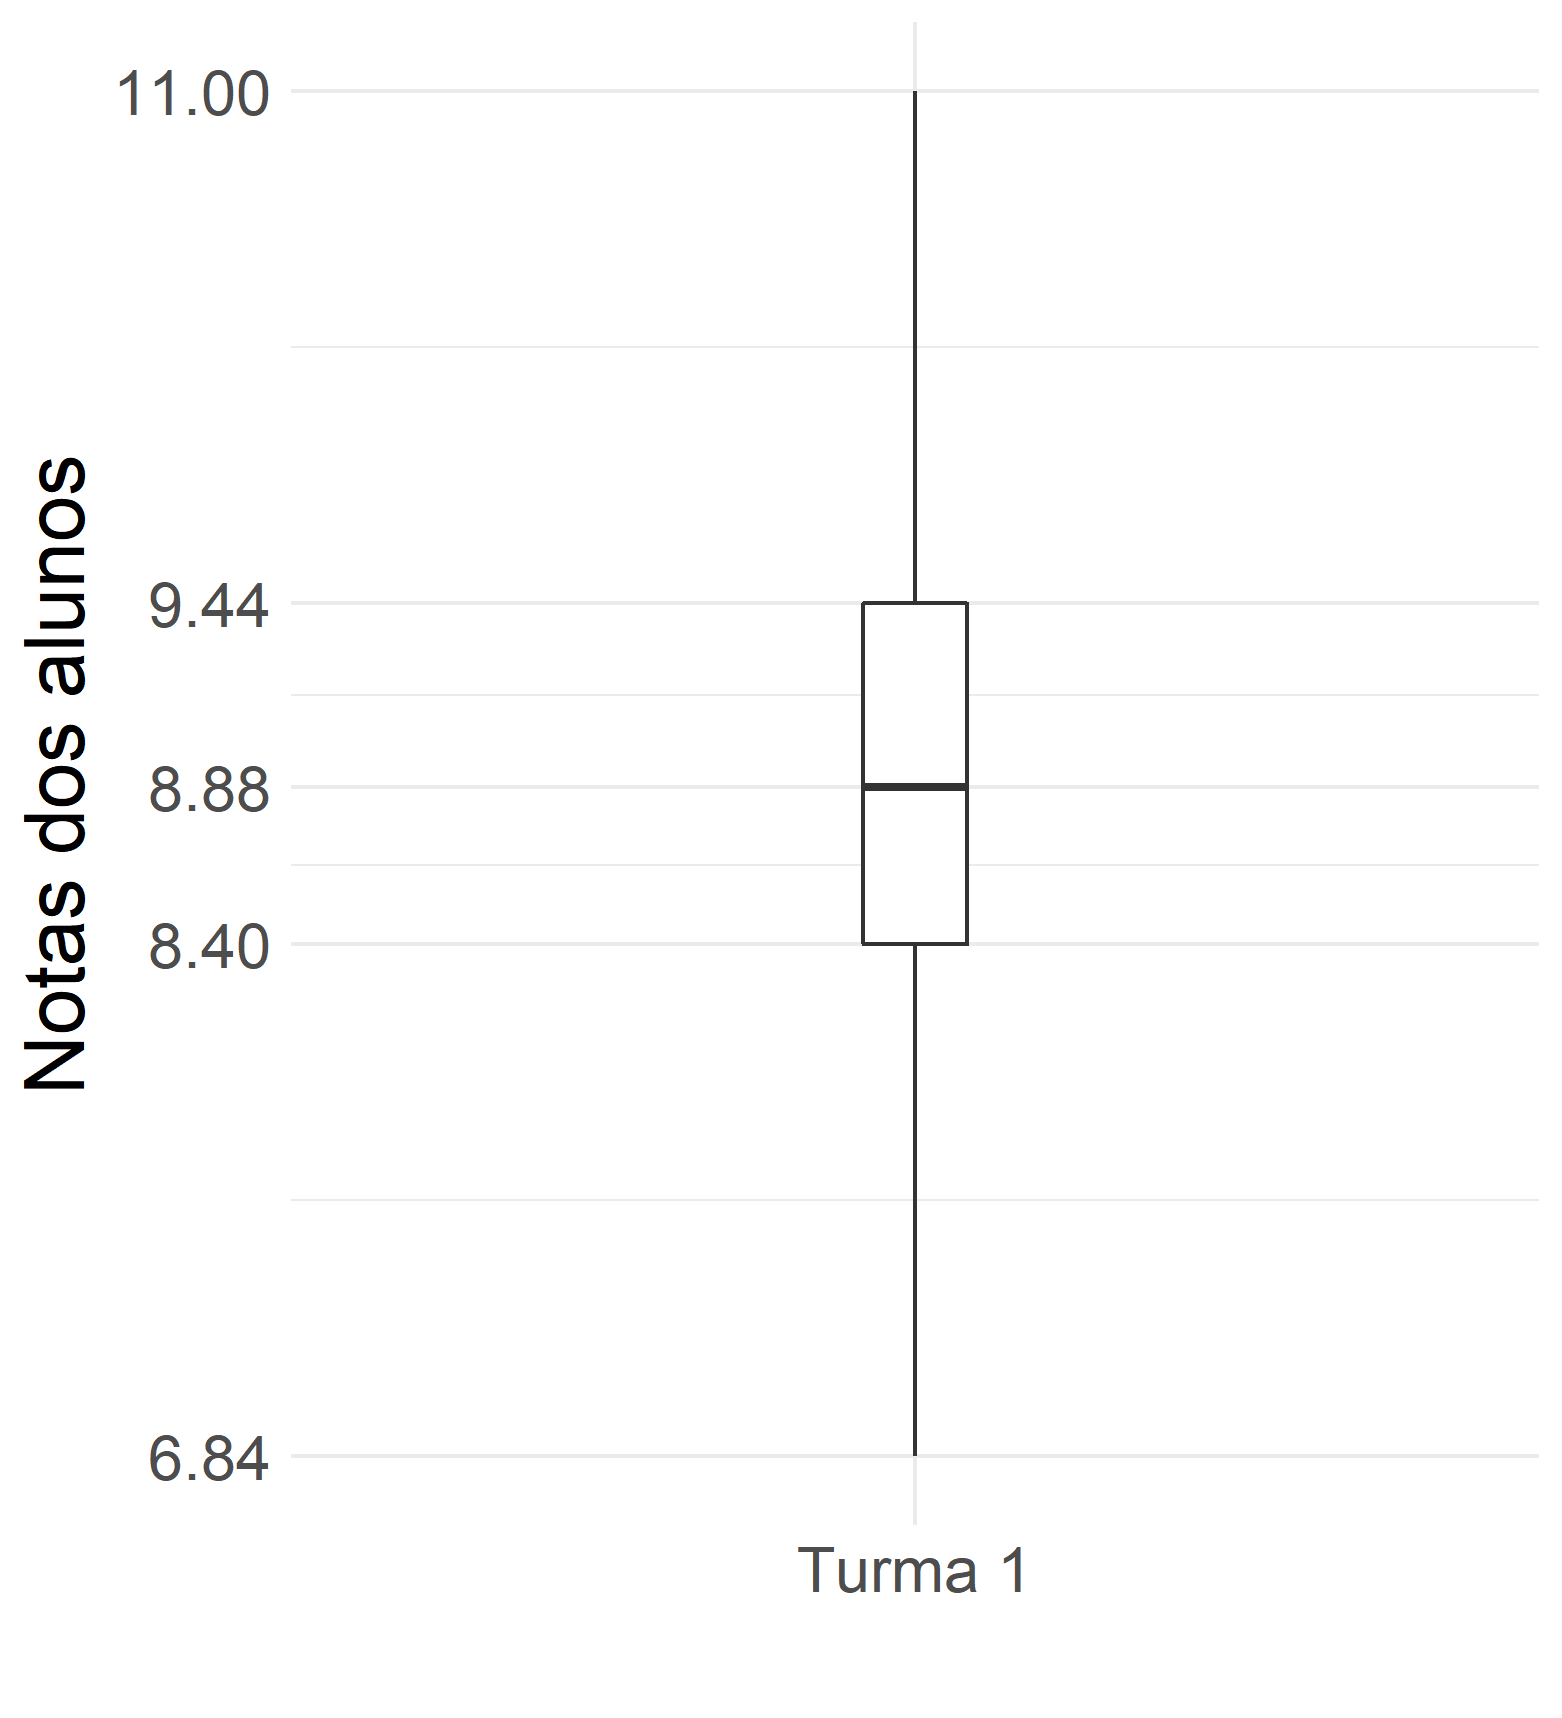
\includegraphics[height=3cm]{asim_boxplot_turma_1.png}
	\end{figure}
\end{frame}

\begin{frame}{Exemplo 1}
	Note que os intervalos $[q_1,q_2]$ e $[q_2,q_3]$  têm $25\%$ dos valores observados, ou seja, os valores estão mais concentrados no intervalo $[q_2, q_3]$ do que $[q_1, q_2]$. 
	Quando isso ocorre, dizemos a variável é assimétrica à esquerda. A figura abaixo ilustra essa idea.
	\begin{figure}[htbp]
		\centering
		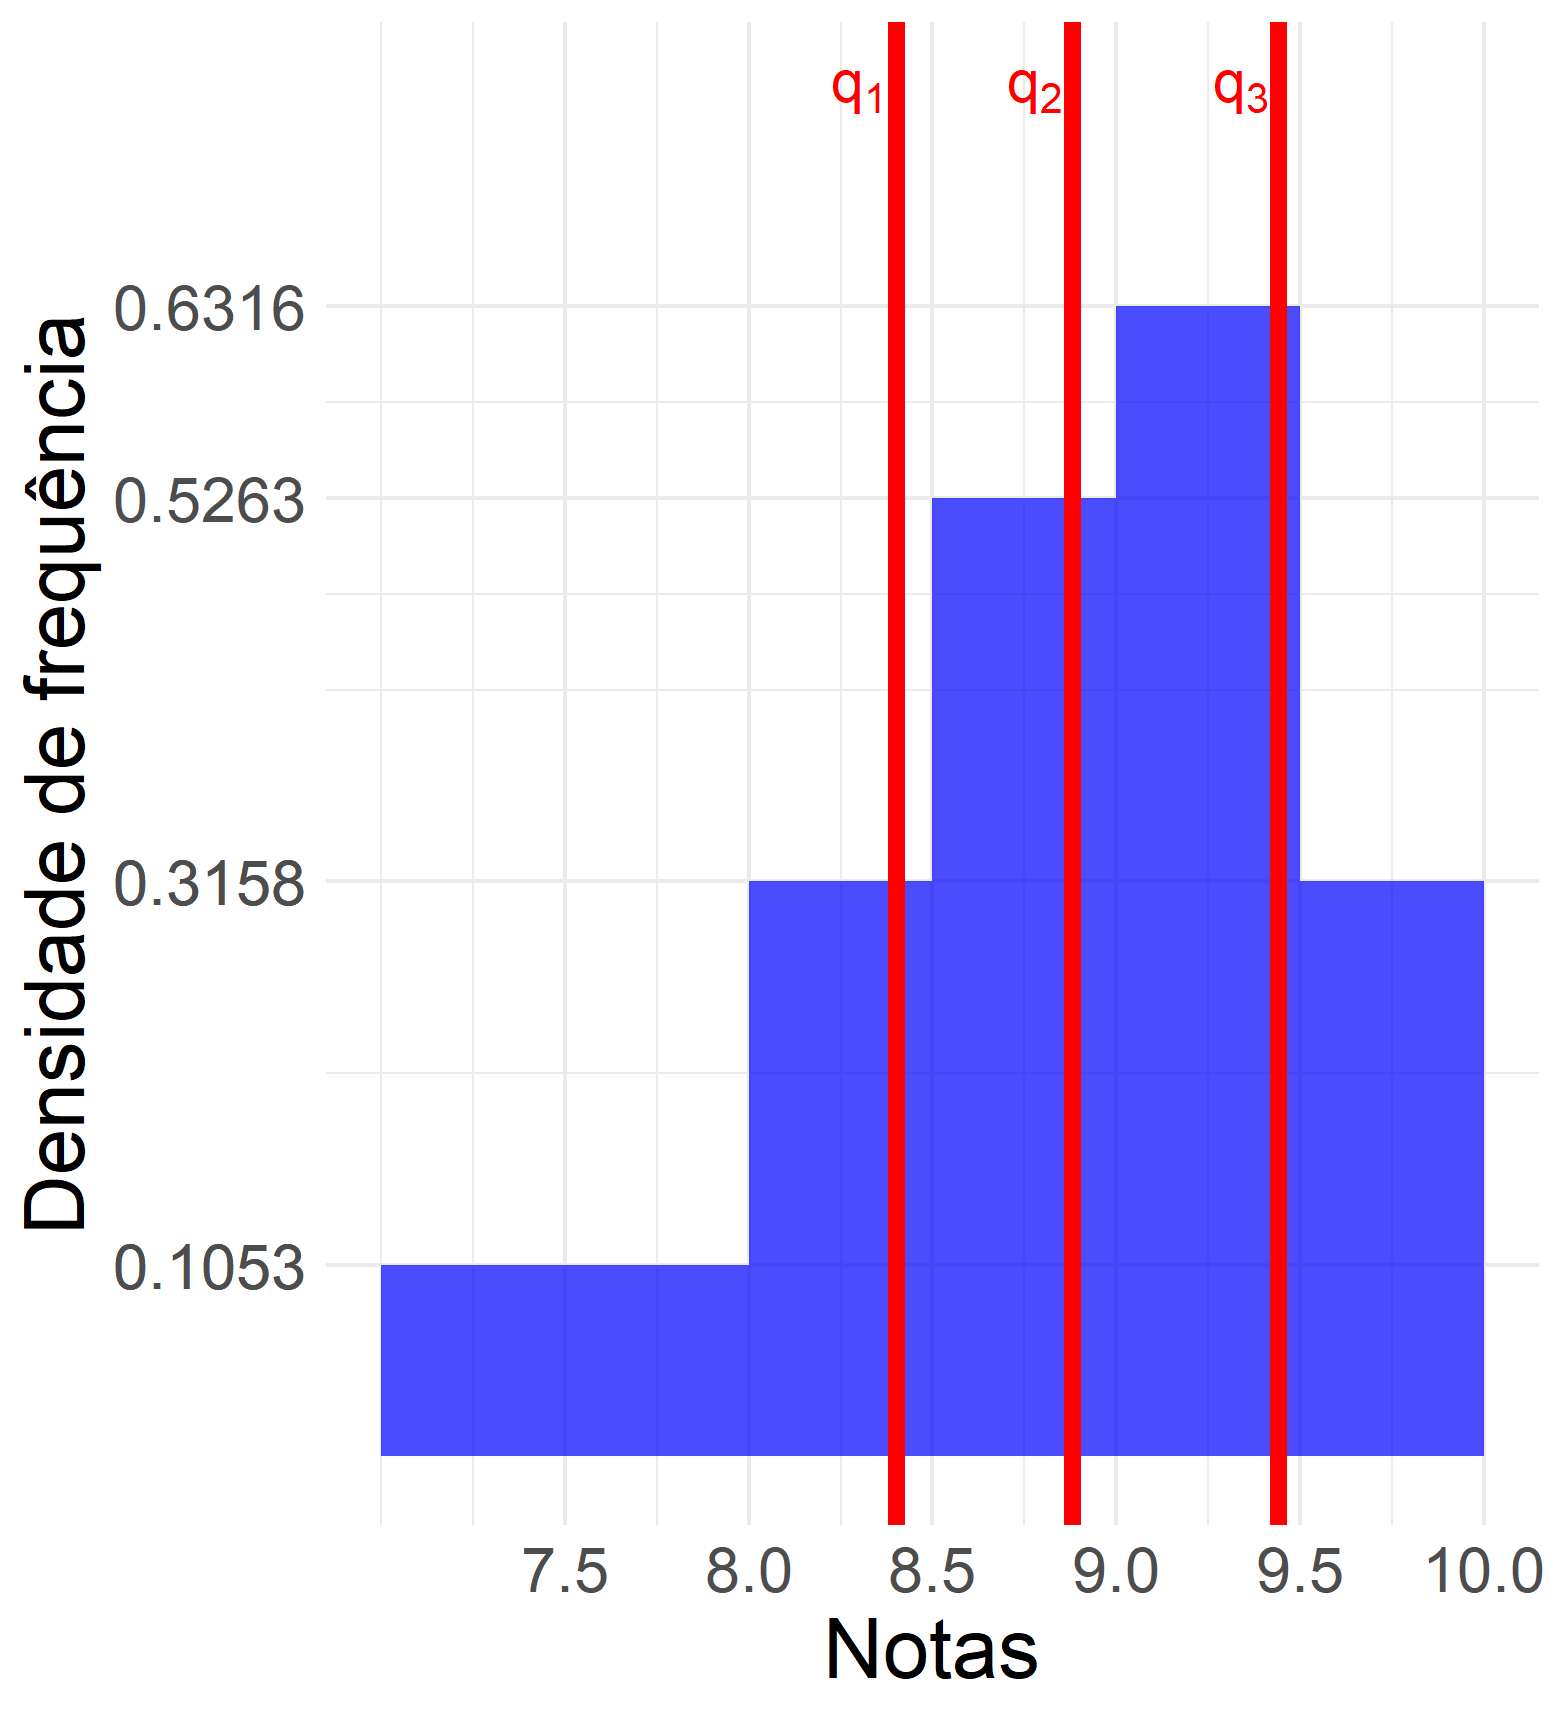
\includegraphics[height=4cm]{asim_histogram_turma_1.png}
	\end{figure}
	Se $q_3-q_2 < q_2 - q_1$, dizemos que a variável tem assimetria a esquerda ou negativa ($q_2$ mais próximo de $q_3$);
\end{frame}

\begin{frame}{Exemplo 2}
Considere as notas da Turma 2 de Estatística Aplicada à Saúde: 2,75; 4,54; 3,08; 4,74; 1,42; 0,61; 1,01; 1,61; 2,8; 8,93; 0,26; 0,58; 2,86; 0,08; 1,21; 1,44; 1,2; 1,24; 0,64. Desenhe o diagrama de caixa.
\vspace{0.25cm}

\textbf{Solução}: Primeiro encontramos as estatísticas de ordem: 
{\tiny		
	\begin{table}[ht]
		\centering
		\begin{tabular}{ccccccccccccccc}
			\toprule[0.05cm]
			$x_{(1)}$ & $x_{(2)}$ & $x_{(3)}$ & $x_{(4)}$ & $x_{(5)}$ & $x_{(6)}$ & $x_{(7)}$ & $x_{(8)}$ & $x_{(9)}$ & $x_{(10)}$ & $x_{(11)}$ & $x_{(12)}$ & $x_{(13)}$ & $x_{(14)}$ & $x_{(15)}$ \\ 
			0,08 & 0,26 & 0,58 & 0,61 & 0,64 & 1,01 & 1,2 & 1,21 & 1,24 & 1,42 & 1,44 & 1,61 & 2,75 & 2,8 & 2,86 \\ \midrule[0.05cm]
			$x_{(16)}$ & $x_{(17)}$ & $x_{(18)}$ & $x_{(19)}$ &   &   &   &   &   &   &   &   &   &   &   \\ 
			3,08 & 4,54 & 4,74 & 8,93 &  &  &  &  &  &  &  &  &  &  &  \\ 
			\bottomrule[0.05cm]
		\end{tabular}
	\end{table}
}

Em seguida, calculamos o primeiro quartil, o segundo quartil, o terceiro quartil, o intervalo interquartílico, o limite superior e o limite inferior:
\begin{align*}
\begin{matrix}
(19+1)\cdot 0,25= 5 & (19+1)\cdot 0,5= 10 & (19+1)\cdot 0,75= 15\\
q_1= x_{(5)} = 0,64 & q_2 = x_{(10)} = 1,42 & q_3 = x_{(15)} = 2,86\\
dq= q_3-q_1 = 2,22 & LS= q_3+1,5\cdot dq = 6,19 &  LI = q_1-1,5\cdot dq=-2,69
\end{matrix}
\end{align*}
\begin{figure}
	\centering
	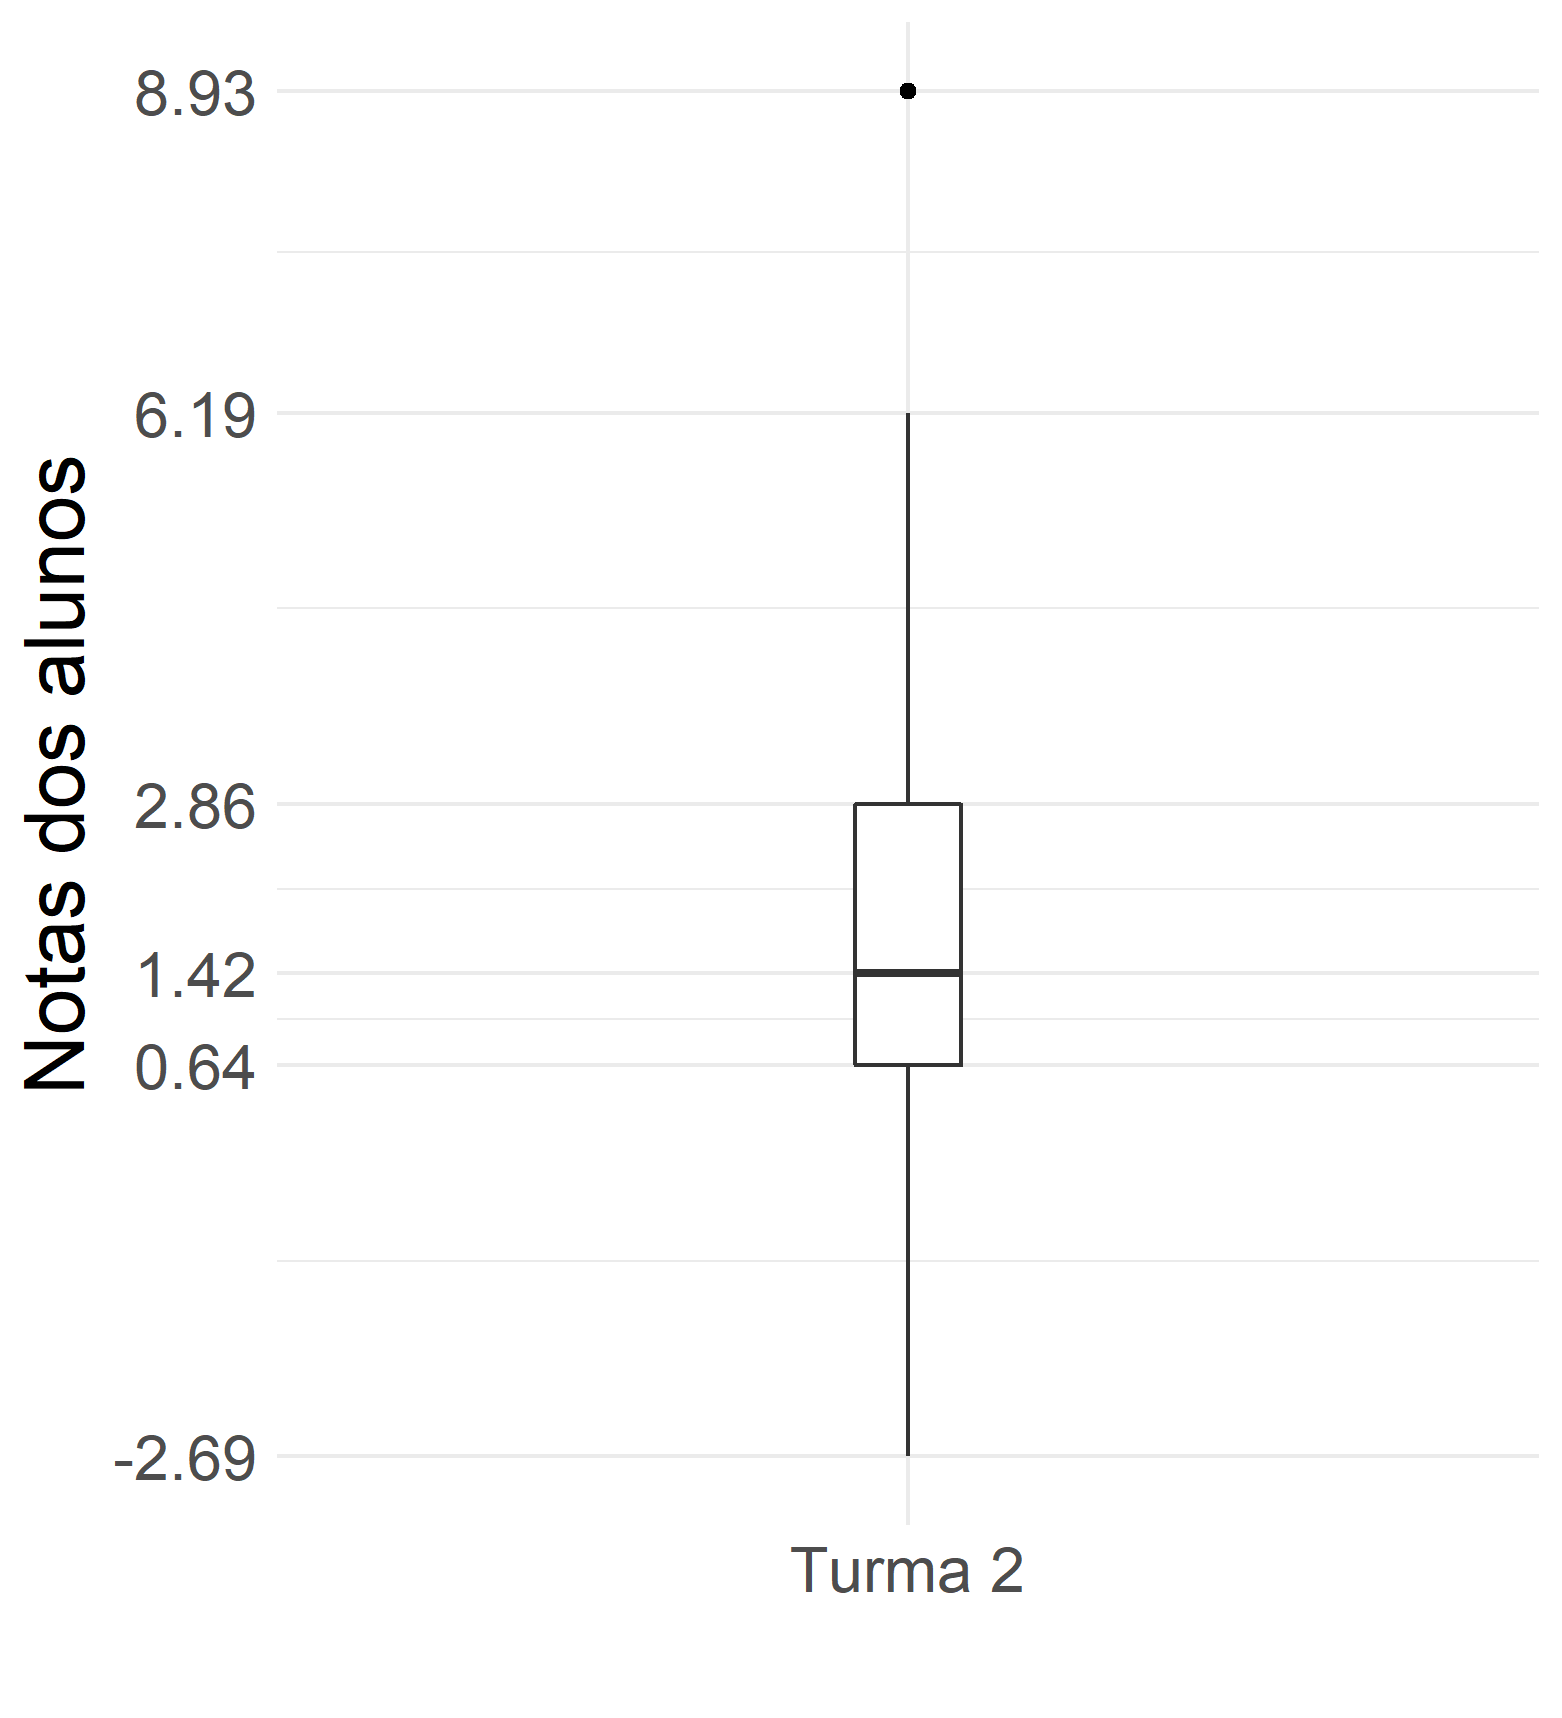
\includegraphics[height=2.5cm]{asim_boxplot_turma_2.png}
\end{figure}
\end{frame}

\begin{frame}{Exemplo 1}
Note que os intervalos $[q_1,q_2]$ e $[q_2,q_3]$  têm $25\%$ dos valores observados, ou seja, os valores estão mais concentrados no intervalo $[q_1, q_2]$ do que $[q_2, q_3]$. 
Quando isso ocorre, dizemos que a variável é assimétrica à direita. A Figura ilustra essa idea.
\begin{figure}[htbp]
\centering
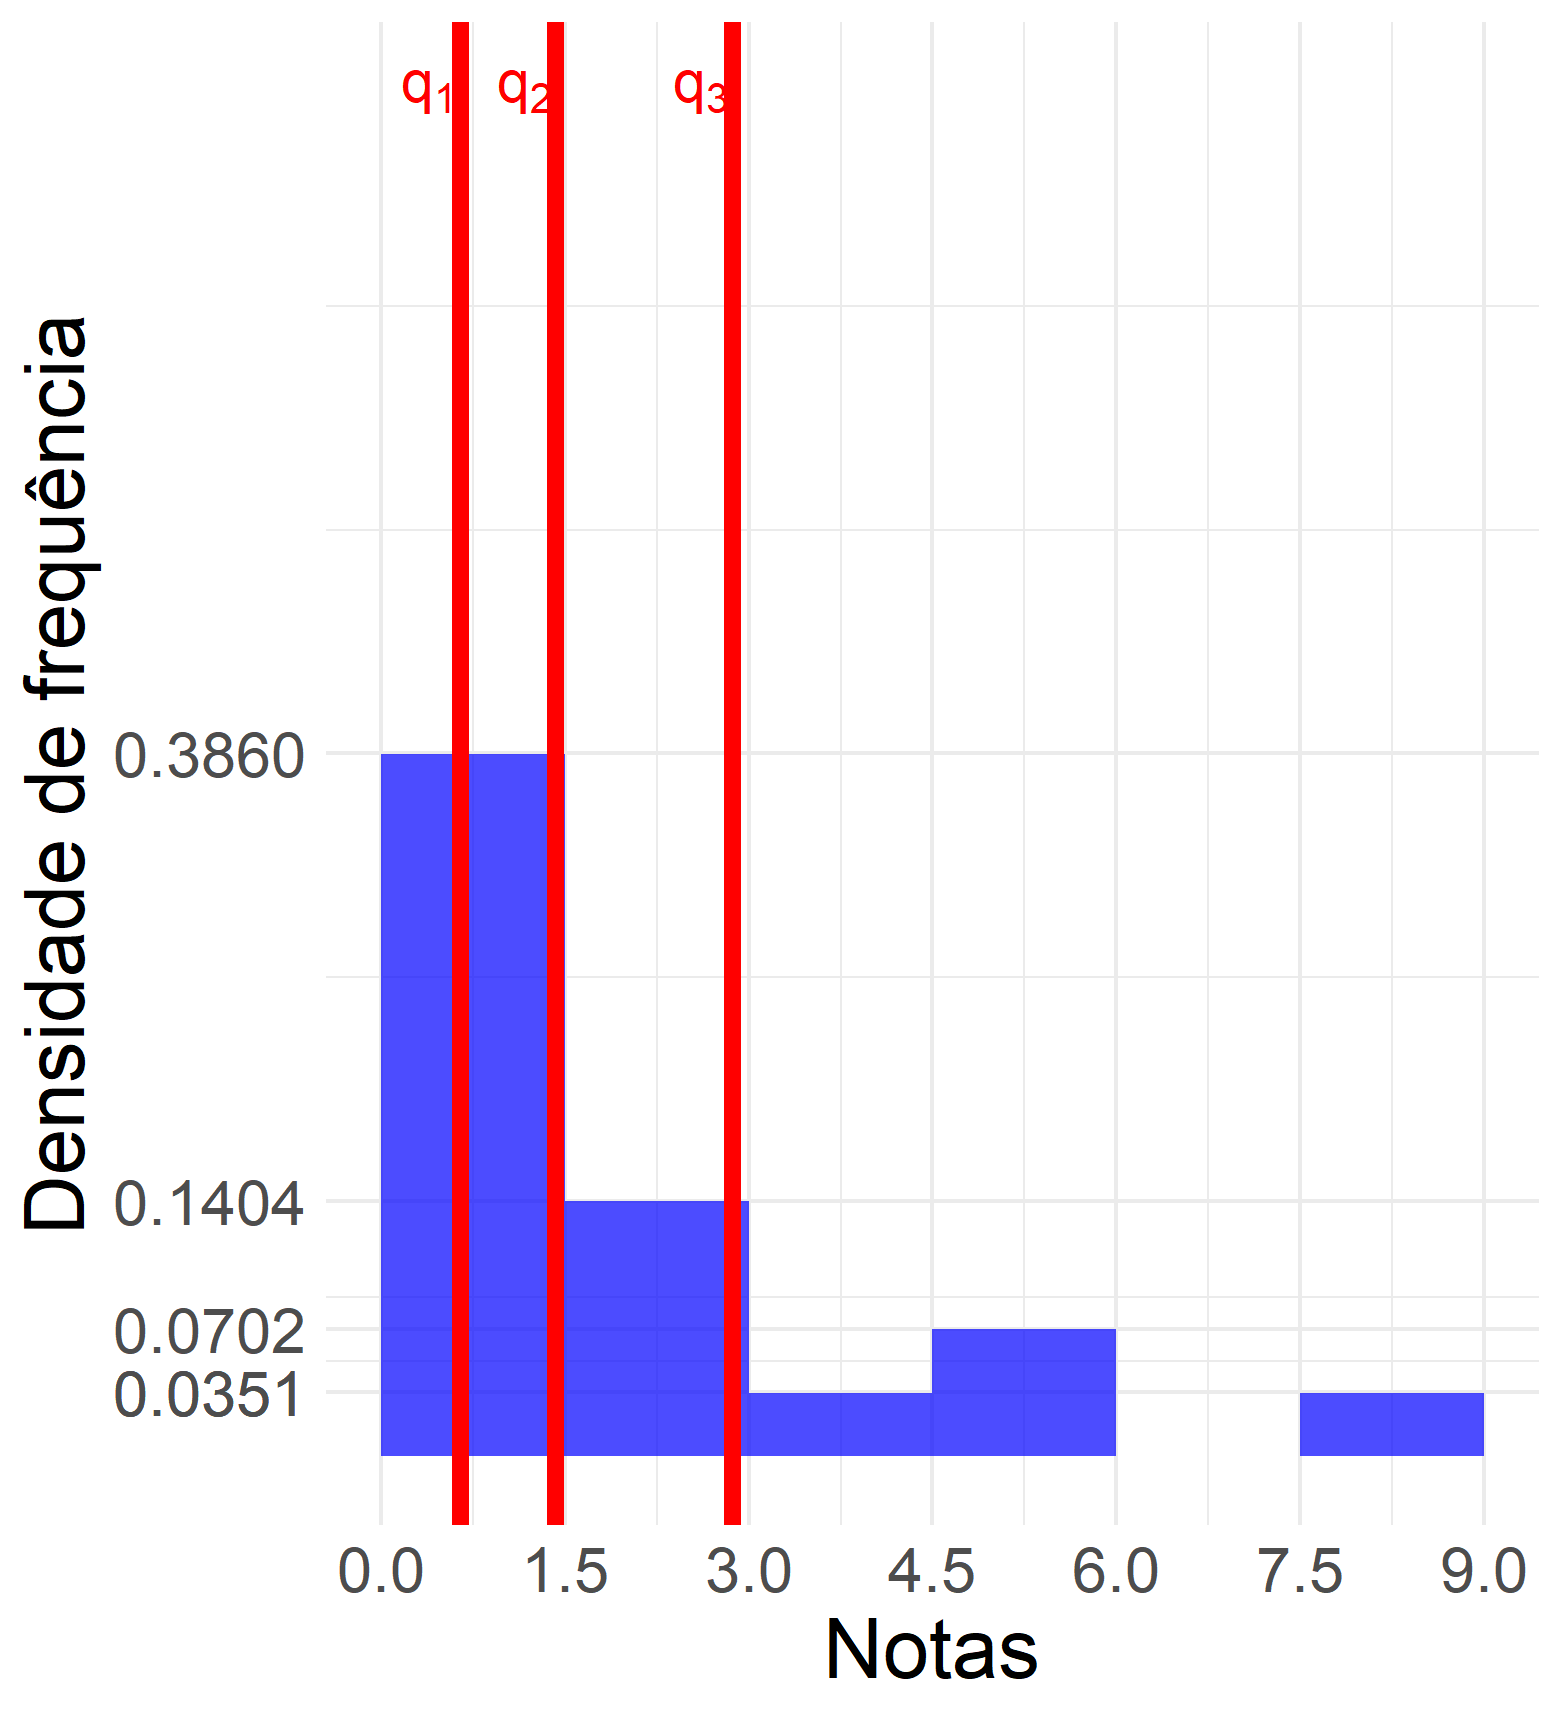
\includegraphics[height=4cm]{asim_histogram_turma_2.png}
\end{figure}
Se $q_2-q_1 < q_3-q_2$, dizemos que a variável tem assimetria à direita ou positiva ($q_2$ mais próximo de $q_1$);
\end{frame}

\begin{frame}{Assimetria}
Inspirados nesses dois exemplos, podemos introduzir uma medida numérica de assimetria, denominado coeficiente de Bowley:
\begin{align*}
	B &= \dfrac{q_3 - 2q_2 +q_1}{q_3-q_1} \\
	&= \dfrac{q_3 - q_2 - (q_2 - q_1)}{q_3 - q_1}
\end{align*}

Note que 
\begin{itemize}
	\item $B \in [-1,1]$;
	\item existe assimetria positiva ou à direita $\iff$ $q_2-q_1 < q_3-q_2$ $\iff$ $B > 0$;
	\item existe assimetria negativa ou à esquerda $\iff$ $q_2-q_1 > q_3-q_2$  $\iff$ $B < 0$;
	\item a variável é simétrica se $B \approx 0$.
\end{itemize}

\begin{block}{Exemplos}
	\begin{itemize}
		\item No exemplo 1, 
		\begin{align*}
		B = \dfrac{q_3 - 2 \cdot q_2 + q_1}{q_3 - q_1} = \dfrac{9,5 - 2 \cdot 9,21 + 8,53}{0,97} = -0.40;
		\end{align*}
		\item No exemplo 2, 
		\begin{align*}
		B = \dfrac{q_3 - 2 \cdot q_2 + q_1}{q_3 - q_1} = \dfrac{7,03 - 2\cdot 6,08 + 5,71}{1,32} = 0,44.
		\end{align*}
	\end{itemize}
\end{block}
\end{frame}
	

% 
% \section{Exercícios em sala de aula}
% 
% \begin{frame}{Exercícios}
% \begin{enumerate}[1.]
%  \item Calcule o primeiro, o segundo e o terceiro quartil para a variável salário usando a tabela de distribuição de frequência;
%  \item Considere as notas finais ($X$) da turma 1 de Estatística Aplicada à Saúde: 4,4; 5,2; 5,3; 5,6; 6,1; 6,4; 7,6; 7,6; 8,0; 8,1; 8,2; 8,9; 9,0; 9,1; 9,8.;
%  Qual a nota que coloca o aluno entre os 10\% melhores alunos da turma? Calcule a média, o desvio médio e o desvio padrão.
%  \item Calcule, a média, o desvio médio, o desvio padrão, o primeiro quartil, o segundo quartil, e o terceiro quartil das 15 maiores cidades do Brasil segundo o IBGE (em 10.000 habitantes).
%  
%  {\small
%  \begin{table}
%   \centering
%   \begin{tabular}{l|c}
%    \toprule[0.05cm]
%    Município & População\\ \midrule[0.05cm]
%    São Paulo & 1125,4\\
%    Rio de Janeiro & 632 \\
%    Salvador & 267,6\\
%    Brasília & 257\\
%    Fortaleza & 245,2\\
%    Belo Horizonte & 235,5\\
%    Manaus & 180,2\\
%    Curitiba & 175,2\\
%    Recife & 153,8\\
%    Porto Alegre & 140,9\\
%    Belém & 139,3\\
%    Goiânia & 130,2\\
%    Guarulhos & 122,2\\
%    Campinas & 108 \\
%    São Gonçalo & 100\\ \bottomrule[0.05cm]
%   \end{tabular}
%  \end{table}
%  }
% \end{enumerate}
% 
%  
% \end{frame}
% 

\end{document}

